\documentclass[hyperref={bookmarks=false},aspectratio=169]{beamer}
\usepackage{hyperref,ragged2e,amsmath,amssymb,url,bm}
\usepackage{graphicx,booktabs,array}
\usepackage{tikz}
\usetikzlibrary{arrows.meta,positioning,calc,shapes.geometric,decorations.pathreplacing,matrix}
\graphicspath{{crops/}}
\usetheme{Goettingen}
% --- Paleta: azul profundo, dorado y papiro crema ---
\definecolor{azul}{HTML}{15437C}
\definecolor{azuloscuro}{HTML}{0B1F3A}
\definecolor{celeste}{HTML}{5694D6}
\definecolor{dorado}{RGB}{196,154,60}
\definecolor{papiro}{RGB}{246,239,220}
\definecolor{gris}{RGB}{70,78,96}
\setbeamercolor{structure}{fg=azul}
\setbeamertemplate{sidebar canvas right}[vertical shading][top=azul,bottom=azuloscuro]
\setbeamercolor{title in sidebar}{fg=dorado}
\setbeamercolor{author in sidebar}{fg=papiro}
\setbeamercolor{section in sidebar}{fg=papiro}
\setbeamercolor{section in sidebar shaded}{fg=dorado!70!papiro}
\setbeamercolor{subsection in sidebar}{fg=papiro}
\setbeamercolor{subsection in sidebar shaded}{fg=dorado!70!papiro}
\let\raggedright\justifying
\setlength{\RaggedRightRightskip}{0pt plus 1fil}
\setbeamertemplate{background canvas}{
\includegraphics[width=\paperwidth,height=\paperheight]{papiro.jpg}}
\setbeamercolor{normal text}{fg=black!88!azuloscuro}
\setbeamercolor{frametitle}{fg=azul}
\setbeamerfont{frametitle}{series=\bfseries}
\setbeamertemplate{section in toc shaded}{\leavevmode{\color{gris}\inserttocsection}\par}
\setbeamercolor{title}{fg=azul}
\setbeamercolor{subtitle}{fg=gris}
\setbeamercolor{item projected}{bg=azul,fg=papiro}
\setbeamertemplate{itemize item}{\small\textcolor{dorado}{$\blacktriangleright$}}
\setbeamertemplate{navigation symbols}{}
% --- Español + hebreo + griego (XeLaTeX) ---
\usepackage[bidi=default]{babel}
\babelprovide[import,main]{spanish}
\babelprovide[import]{hebrew}
\babelprovide[import]{ancientgreek}
\babelfont[hebrew]{sf}[Path=fonts/, BoldFont=NotoHebrewSans-700.ttf]{NotoHebrewSans-400.ttf}
\babelfont[hebrew]{rm}[Path=fonts/, BoldFont=NotoHebrewSans-700.ttf]{NotoHebrewSans-400.ttf}
\babelfont[ancientgreek]{sf}[Path=fonts/]{GFSPorson.otf}
\babelfont[ancientgreek]{rm}[Path=fonts/]{GFSPorson.otf}
\newcommand{\heb}[1]{\mbox{\foreignlanguage{hebrew}{#1}}}
\newcommand{\grc}[1]{\foreignlanguage{ancientgreek}{#1}}
\newcommand{\SENOR}{S{\fontsize{0.78em}{1em}\selectfont EÑOR}}
% --- Citas (cuadro de un solo color), imágenes, referencias ---
\usepackage[most]{tcolorbox}
\newtcolorbox{cita}[1][]{enhanced, colback=azul!7!papiro, opacityback=0.85, colframe=azul,
  boxrule=0pt, leftrule=2.5pt, arc=0pt, left=6pt, right=6pt, top=4pt, bottom=4pt,
  before skip=4pt, after skip=6pt, fontupper=\small\itshape, #1}
\newcommand{\fuente}[1]{\par\hfill{\upshape\bfseries\footnotesize\textcolor{azul}{#1}}}
\makeatletter
\newcommand{\fotolado}[2]{%
  \begin{tikzpicture}[remember picture,overlay]
    \node[anchor=north east,inner sep=0pt] (foto) at ([xshift=-\beamer@sidebarwidth]current page.north east)
      {\includegraphics[height=\paperheight]{#1}};
    \node[anchor=south east,inner sep=2pt,text=papiro,fill=azuloscuro,fill opacity=0.6,text opacity=1,
      font=\fontsize{4.5}{5.5}\selectfont,align=right,text width=4.2cm] at ([xshift=-3pt,yshift=3pt]foto.south east)
      {\textit{Nota.} #2};
  \end{tikzpicture}}
\makeatother
\newcommand{\refapa}[1]{\par{\RaggedRight\hangindent=1.2em\hangafter=1\noindent #1\par}\vspace{3pt}}
\usepackage{xurl}\urlstyle{same}
\newcommand{\destacar}[1]{\textbf{\textcolor{azul}{#1}}}
\newcommand{\precision}[1]{{\footnotesize\color{gris}\textbf{Precisión:} #1}}
\tikzset{caja/.style={draw=azul,line width=0.8pt,fill=papiro,fill opacity=0.92,text opacity=1,rounded corners=3pt,inner sep=5pt,font=\scriptsize}}
\title[La inmutabilidad de Dios]{\bfseries{La inmutabilidad de Dios}}
\subtitle{``Porque yo \SENOR{} no cambio'' (Mal 3:6)}
\author{}\institute{}\date{}
\titlegraphic{
\includegraphics[width=0.80\linewidth,height=0.36\textheight,keepaspectratio]{portada.jpg}\\[-1pt]
  {\fontsize{5}{6}\selectfont\color{gris}\textit{Nota.} Elaboración propia: Mal 3:6a en texto hebreo consonántico (BHS).}}
\AtBeginSection[]{\begin{frame}\frametitle{Contenidos}\tableofcontents[currentsection]\end{frame}}
\begin{document}
\frame{\titlepage}

\begin{frame}\frametitle{Contenidos}\tableofcontents\end{frame}

% ------------------------------------------------------------------
\section{Contexto}

\begin{frame}{Todo cambia}
\begin{columns}[c,onlytextwidth]
\begin{column}{0.52\textwidth}
\begin{cita}Desde el principio tú fundaste la tierra, y los cielos son obra de tus manos. Ellos perecerán, mas tú permanecerás; y todos ellos como una vestidura se envejecerán; como un vestido los mudarás, y serán mudados; pero tú eres el mismo, y tus años no se acabarán.\fuente{(Sal 102:25--27 [102:26--28], RVR1960)}\end{cita}
\end{column}
\begin{column}{0.46\textwidth}
\centering
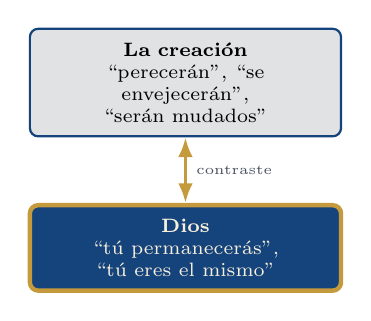
\begin{tikzpicture}[font=\scriptsize]
 \node[caja,text width=3.6cm,align=center,fill=gris!18] (c) at (0,1.5) {\textbf{La creación}\\ ``perecerán'', ``se envejecerán'', ``serán mudados''};
 \node[draw=dorado,line width=1.6pt,fill=azul,text=papiro,rounded corners=3pt,text width=3.6cm,align=center,inner sep=5pt] (d) at (0,-0.6) {\textbf{Dios}\\ ``tú permanecerás'', ``tú eres el mismo''};
 \draw[{Latex[length=2.5mm]}-{Latex[length=2.5mm]},dorado,line width=1.2pt] (c)--(d) node[midway,right,font=\tiny,text=gris]{contraste};
\end{tikzpicture}\par\medskip
\small El salmo no define a Dios en abstracto: lo pone \destacar{frente a la creación}, que envejece como ropa usada.
\end{column}
\end{columns}
\end{frame}

\begin{frame}{¿Qué significa ``inmutable''?}
\begin{columns}[c,onlytextwidth]
\begin{column}{0.50\textwidth}\small
\begin{itemize}
\item ``Inmutable'' significa \destacar{que no cambia}.
\item En la Biblia no significa que Dios sea estático, frío o incapaz de relacionarse.
\item Significa que Dios no cambia en su \destacar{esencia}, en su \destacar{carácter} ni en su \destacar{fidelidad}.
\end{itemize}
\begin{tcolorbox}[colback=papiro,colframe=dorado,boxrule=1.2pt,arc=3pt]
\small Dios no cambia en quién es, pero sí puede cambiar lo que hace, sin dejar de ser fiel a su carácter justo y misericordioso.
\end{tcolorbox}
\end{column}
\begin{column}{0.48\textwidth}
\centering
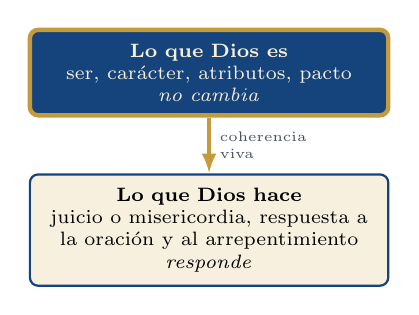
\begin{tikzpicture}[font=\scriptsize]
 \node[draw=dorado,line width=1.6pt,fill=azul,text=papiro,rounded corners=3pt,text width=4.2cm,align=center,inner sep=5pt] (s) at (0,1.6) {\textbf{Lo que Dios es}\\ ser, carácter, atributos, pacto\\ \emph{no cambia}};
 \node[caja,text width=4.2cm,align=center] (h) at (0,-0.4) {\textbf{Lo que Dios hace}\\ juicio o misericordia, respuesta a la oración y al arrepentimiento\\ \emph{responde}};
 \draw[-{Latex[length=2.5mm]},dorado,line width=1.2pt] (s)--(h) node[midway,right,font=\tiny,text=gris,text width=1.6cm]{coherencia viva};
\end{tikzpicture}
\end{column}
\end{columns}
\end{frame}

\begin{frame}{Un atributo de identidad}
\begin{columns}[c,onlytextwidth]
\begin{column}{0.52\textwidth}\small
\begin{itemize}
\item La serie clasifica la inmutabilidad entre los atributos de \destacar{Identidad}: responde a la pregunta \emph{¿quién es Dios?}
\item Es \destacar{incomunicable}: solo Dios es el mismo para siempre. ``Criatura y mutabilidad son términos correlativos'' (Pink, 2020, cap. 7).
\item Tiene un \destacar{reflejo comunicable}: la constancia del justo, ``que aun jurando en daño suyo, no por eso cambia'' (Sal 15:4).
\end{itemize}
\end{column}
\begin{column}{0.46\textwidth}
\scriptsize\renewcommand{\arraystretch}{1.2}
\begin{tabular}{@{}>{\RaggedRight\arraybackslash}p{1.9cm}>{\RaggedRight\arraybackslash}p{3.6cm}@{}}
\toprule
\textbf{Clase} & \textbf{Atributos} \\ \midrule
Ser & Uno, Amor, Espíritu \\
\destacar{Identidad} & Santo, Eterno, Soberano, Justo, \destacar{Inmutable}, Omnipotente, Omnipresente, Omnisciente \\
Relación & Sabiduría, Verdadero, Misericordioso, Fiel, Celo, Ira santa, Bondad, Paciencia, Gracia \\
\bottomrule
\end{tabular}
\end{column}
\end{columns}\par\smallskip
\precision{clasificación según el plan de la serie; ``incomunicable con reflejo comunicable'' es propuesta de esta presentación.}
\end{frame}

\begin{frame}{``Inmutable'' en la RVR1960}
\begin{columns}[c,onlytextwidth]
\begin{column}{0.44\textwidth}\footnotesize
\begin{itemize}
\item La palabra ``inmutable'' es \destacar{rara}: 3 veces, todas en Hebreos (6:17, 18; 7:24).
\item El AT lo dice con frases: ``no cambio'', ``tú eres el mismo'', ``permanecerás'', ``no se arrepentirá''.
\item El verbo que más discusión trae es \heb{נחם} \emph{najam}, ``arrepentirse'': con Dios como sujeto aparece en unos \textbf{34 versículos}.
\end{itemize}
\end{column}
\begin{column}{0.54\textwidth}
\scriptsize\renewcommand{\arraystretch}{1.12}
\begin{tabular}{@{}>{\RaggedRight\arraybackslash}p{2.9cm}>{\RaggedRight\arraybackslash}p{3.2cm}@{}}
\toprule
\textbf{Expresión RVR1960} & \textbf{Textos} \\ \midrule
``inmutabilidad'', ``inmutable(s)'' & He 6:17, 18; 7:24 \\
``no cambio'' & Mal 3:6 \\
``tú eres el mismo'', ``es el mismo'' & Sal 102:27; He 1:12; 13:8 \\
``no hay mudanza'' & Stg 1:17 \\
``irrevocables'' & Ro 11:29 \\
``no se arrepentirá'' (de Dios) & Nm 23:19; 1 S 15:29; Sal 110:4 \\
``se arrepintió'' (de Dios) & Gn 6:6; Éx 32:14; Jon 3:10\ldots \\
\bottomrule
\end{tabular}
\end{column}
\end{columns}\par\smallskip
\precision{conteo propio en la RVR1960 sin títulos de sección y en la BHS por raíz consonántica; verificar en e-Sword.}
\end{frame}

% ------------------------------------------------------------------
\section{Malaquías}

\begin{frame}{Texto ancla: Mal 3:6}
\fotolado{panel_malaquias3.jpg}{Elaboración propia: Mal 3:6 en texto hebreo consonántico (BHS).}
\begin{columns}[c,onlytextwidth]
\begin{column}{0.58\textwidth}
\begin{cita}Porque yo \SENOR{} no cambio; por esto, hijos de Jacob, no habéis sido consumidos.\fuente{(Mal 3:6, RVR1960)}\end{cita}
\begin{center}\heb{כִּי אֲנִי יְהוָה לֹא שָׁנִיתִי}\\[2pt]\heb{וְאַתֶּם בְּנֵי־יַעֲקֹב לֹא כְלִיתֶם}\end{center}
\small El contexto es el \destacar{pacto}: si Dios cambiara, Israel ya habría sido destruido. Su fidelidad es la prueba de su inmutabilidad.
\end{column}
\begin{column}{0.40\textwidth}\end{column}
\end{columns}
\end{frame}

\begin{frame}{Mal 3:6: la palabra}
\scriptsize\renewcommand{\arraystretch}{1.15}
\begin{tabular}{@{}>{\RaggedRight\arraybackslash}p{2.8cm}>{\RaggedRight\arraybackslash}p{1.1cm}>{\RaggedRight\arraybackslash}p{8.0cm}@{}}
\toprule
\textbf{Término} & \textbf{Raíz} & \textbf{Sentido} \\ \midrule
\heb{אֲנִי יְהוָה} \emph{aní YHWH} & --- & ``yo, el \SENOR'': Dios habla en primera persona y con su Nombre de pacto. \\
\heb{לֹא שָׁנִיתִי} \emph{lo shaníti} & \heb{שׁנה} & ``no he cambiado'': perfecto, una condición que se mantiene. La raíz significa ``cambiar, ser distinto'' y también ``repetir'' (de ahí \heb{שָׁנָה} \emph{shaná}, ``año''). \\
\heb{בְּנֵי־יַעֲקֹב} \emph{bené Ya'aqov} & --- & ``hijos de Jacob'': el nombre del patriarca que engañó y fue cambiado (Gn 32:28). \\
\heb{לֹא כְלִיתֶם} \emph{lo jelitem} & \heb{כלה} & ``no habéis sido acabados, consumidos''. \\
\bottomrule
\end{tabular}\par\medskip
\begin{columns}[t,onlytextwidth]
\begin{column}{0.49\textwidth}\small
\textbf{LXX:} \grc{ἐγὼ κύριος ὁ θεὸς ὑμῶν καὶ οὐκ ἠλλοίωμαι}: ``yo soy el Señor vuestro Dios, y no he sido alterado''. \grc{ἀλλοιόω} es ``volverse otro''.
\end{column}
\begin{column}{0.49\textwidth}\small
La misma raíz \heb{שׁנה} describe a los hombres: ``no te entremetas con los \destacar{veleidosos}'' (\heb{שׁוֹנִים} \emph{shonim}, Pr 24:21), los que cambian.
\end{column}
\end{columns}
\end{frame}

\begin{frame}{Mal 3: el contexto}
\centering
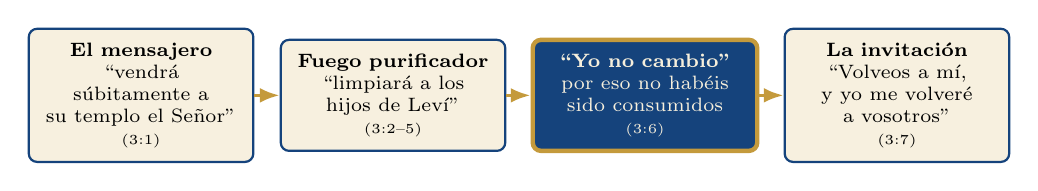
\begin{tikzpicture}[font=\scriptsize]
 \node[caja,text width=2.5cm,align=center] (a) at (0,0) {\textbf{El mensajero}\\ ``vendrá súbitamente a su templo el Señor''\\ {\tiny(3:1)}};
 \node[caja,text width=2.5cm,align=center] (b) at (3.2,0) {\textbf{Fuego purificador}\\ ``limpiará a los hijos de Leví''\\ {\tiny(3:2--5)}};
 \node[draw=dorado,line width=1.6pt,fill=azul,text=papiro,rounded corners=3pt,text width=2.5cm,align=center,inner sep=5pt] (c) at (6.4,0) {\textbf{``Yo no cambio''}\\ por eso no habéis sido consumidos\\ {\tiny(3:6)}};
 \node[caja,text width=2.5cm,align=center] (d) at (9.6,0) {\textbf{La invitación}\\ ``Volveos a mí, y yo me volveré a vosotros''\\ {\tiny(3:7)}};
 \draw[-{Latex[length=2.5mm]},dorado,line width=1.2pt] (a)--(b); \draw[-{Latex[length=2.5mm]},dorado,line width=1.2pt] (b)--(c); \draw[-{Latex[length=2.5mm]},dorado,line width=1.2pt] (c)--(d);
\end{tikzpicture}\par\medskip
\begin{columns}[t,onlytextwidth]
\begin{column}{0.52\textwidth}
\begin{cita}Desde los días de vuestros padres os habéis apartado de mis leyes, y no las guardasteis. Volveos a mí, y yo me volveré a vosotros, ha dicho \SENOR{} de los ejércitos.\fuente{(Mal 3:7, RVR1960)}\end{cita}
\end{column}
\begin{column}{0.46\textwidth}\small
\begin{itemize}
\item En un mismo pasaje: Dios \destacar{no cambia} (v. 6) y Dios \destacar{se vuelve} (\heb{וְאָשׁוּבָה}, v. 7).
\item La inmutabilidad no impide la relación: es la \destacar{base} de la invitación.
\end{itemize}
\end{column}
\end{columns}
\end{frame}

\begin{frame}{``No habéis sido consumidos''}
\begin{columns}[t,onlytextwidth]
\begin{column}{0.50\textwidth}
\begin{cita}Por la misericordia de \SENOR{} no hemos sido consumidos, porque nunca decayeron sus misericordias. Nuevas son cada mañana; grande es tu fidelidad.\fuente{(Lm 3:22--23, RVR1960)}\end{cita}
\begin{center}\heb{חַסְדֵי יְהוָה כִּי לֹא־תָמְנוּ כִּי לֹא־כָלוּ רַחֲמָיו}\end{center}
\end{column}
\begin{column}{0.48\textwidth}\small
\begin{itemize}
\item Malaquías: ``no habéis sido \destacar{consumidos}'' (\heb{לֹא כְלִיתֶם}).
\item Lamentaciones: sus misericordias ``nunca \destacar{decayeron}'' (\heb{לֹא־כָלוּ}).
\item La misma raíz \heb{כלה}: Israel no se acaba \destacar{porque} la misericordia de Dios no se acaba.
\end{itemize}
\precision{la conexión léxica entre los dos textos es observación propia.}
\end{column}
\end{columns}
\end{frame}

% ------------------------------------------------------------------
\section{Salmo 102}

\begin{frame}{``Pero tú eres el mismo''}
\fotolado{panel_salmo102.jpg}{Elaboración propia: Sal 102:26--27 [102:27--28] en texto hebreo consonántico (BHS).}
\begin{columns}[c,onlytextwidth]
\begin{column}{0.58\textwidth}
\begin{cita}Ellos perecerán, mas tú permanecerás; y todos ellos como una vestidura se envejecerán; como un vestido los mudarás, y serán mudados; pero tú eres el mismo, y tus años no se acabarán.\fuente{(Sal 102:26--27 [102:27--28], RVR1960)}\end{cita}
\small El encabezado lo presenta como ``Oración del que sufre, cuando está angustiado'' (102:1). El orante, cuyos días ``se han consumido como humo'' (v. 3), se aferra al Dios cuyos años no se acaban.
\end{column}
\begin{column}{0.40\textwidth}\end{column}
\end{columns}
\end{frame}

\begin{frame}{Sal 102:26--27: la palabra}
\begin{center}\heb{הֵמָּה יֹאבֵדוּ וְאַתָּה תַעֲמֹד וְכֻלָּם כַּבֶּגֶד יִבְלוּ}\\[2pt]\heb{כַּלְּבוּשׁ תַּחֲלִיפֵם וְיַחֲלֹפוּ וְאַתָּה־הוּא וּשְׁנוֹתֶיךָ לֹא יִתָּמּוּ}\end{center}
\scriptsize\renewcommand{\arraystretch}{1.13}
\begin{tabular}{@{}>{\RaggedRight\arraybackslash}p{2.9cm}>{\RaggedRight\arraybackslash}p{1.1cm}>{\RaggedRight\arraybackslash}p{7.9cm}@{}}
\toprule
\textbf{Término} & \textbf{Raíz} & \textbf{Sentido} \\ \midrule
\heb{תַעֲמֹד} \emph{ta'amod} & \heb{עמד} & ``permanecerás'', literalmente ``estarás en pie'': Dios sigue de pie cuando todo cae. \\
\heb{יִבְלוּ} \emph{yivlú} & \heb{בלה} & ``se envejecerán'', se gastarán como tela. \\
\heb{תַּחֲלִיפֵם וְיַחֲלֹפוּ} & \heb{חלף} & ``los mudarás, y serán mudados'': Dios cambia la creación como quien cambia de ropa; él no es cambiado. \\
\heb{וְאַתָּה־הוּא} \emph{ve'atá hu} & --- & ``y tú (eres) él'': ``tú eres el mismo''. Sin verbo: identidad pura. \\
\heb{לֹא יִתָּמּוּ} \emph{lo yitammu} & \heb{תמם} & ``no se acabarán'': no llegan a término. \\
\bottomrule
\end{tabular}\par\smallskip
\small El verbo \heb{חלף} es activo para Dios y pasivo para la creación: \destacar{él cambia las cosas; las cosas no lo cambian a él}.
\end{frame}

\begin{frame}{``Tú eres él'': \emph{atá hu}, \emph{aní hu}}
\centering
\begin{tikzpicture}[font=\scriptsize]
 \node[caja,text width=2.6cm,align=center] (a) at (0,0) {\heb{אֲנִי אֲנִי הוּא}\\ ``yo, yo soy''\\ {\tiny(Dt 32:39)}};
 \node[caja,text width=2.6cm,align=center] (b) at (3.3,0) {\heb{אֲנִי־הוּא}\\ ``yo mismo con los postreros''\\ {\tiny(Is 41:4; 43:10; 48:12)}};
 \node[draw=dorado,line width=1.6pt,fill=azul,text=papiro,rounded corners=3pt,text width=2.6cm,align=center,inner sep=5pt] (c) at (6.6,0) {\heb{וְאַתָּה־הוּא}\\ ``tú eres el mismo''\\ {\tiny(Sal 102:27)}};
 \node[caja,text width=2.6cm,align=center] (d) at (9.9,0) {\grc{σὺ δὲ ὁ αὐτὸς εἶ}\\ LXX Sal 101:28\\ {\tiny(= He 1:12)}};
 \draw[-{Latex[length=2.5mm]},dorado,line width=1.1pt] (a)--(b); \draw[-{Latex[length=2.5mm]},dorado,line width=1.1pt] (b)--(c); \draw[-{Latex[length=2.5mm]},dorado,line width=1.1pt] (c)--(d);
\end{tikzpicture}\par\medskip
\begin{columns}[t,onlytextwidth]
\begin{column}{0.52\textwidth}
\begin{cita}Yo \SENOR, el primero, y yo mismo con los postreros.\fuente{(Is 41:4, RVR1960)}\end{cita}
\end{column}
\begin{column}{0.46\textwidth}\small
\heb{הוּא} \emph{hu}, ``él'', funciona casi como un nombre: el que fue, es y será \destacar{el mismo}. La LXX traduce \emph{aní hu} con \grc{ἐγώ εἰμι} y \emph{atá hu} con \grc{σὺ ὁ αὐτὸς εἶ}.
\end{column}
\end{columns}
\precision{la lectura de \emph{hu} como designación de la identidad divina es una interpretación frecuente en los comentarios; no es un nombre propio en el texto.}
\end{frame}

% ------------------------------------------------------------------
\section{La palabra}

\begin{frame}{El espectro: hebreo}
\scriptsize\renewcommand{\arraystretch}{1.12}
\begin{tabular}{@{}>{\RaggedRight\arraybackslash}p{2.7cm}>{\RaggedRight\arraybackslash}p{3.1cm}>{\RaggedRight\arraybackslash}p{2.6cm}>{\RaggedRight\arraybackslash}p{3.3cm}@{}}
\toprule
\textbf{Término} & \textbf{Sentido} & \textbf{RVR1960} & \textbf{Textos} \\ \midrule
\heb{שָׁנָה} \emph{shaná} & cambiar, alterar; repetir & cambio, mudaré & Mal 3:6; Sal 89:34 [89:35]; Pr 24:21 \\
\heb{מוּר} \emph{mur} & cambiar, permutar & cambia & Sal 15:4; Lv 27:10 \\
\heb{חָלַף} \emph{jalaf} & pasar, cambiar (ropa) & mudarás, serán mudados & Sal 102:26 [102:27] \\
\heb{עָמַד} \emph{amad} & estar en pie, permanecer & permanecerás, permanecerá & Sal 102:26; 33:11 \\
\heb{קוּם} \emph{qum} & levantarse, mantenerse & permanece & Is 40:8; 46:10 \\
\heb{נחם} \emph{najam} (nifal) & lamentar, desistir; consolarse & arrepentirse, pesar, dolerse & Gn 6:6; 1 S 15:29; Jon 3:10 \\
\heb{צוּר} \emph{tsur} & roca, peña & Roca & Dt 32:4, 15, 18, 30--31 \\
\bottomrule
\end{tabular}\par\medskip
\begin{cita}No olvidaré mi pacto, ni mudaré lo que ha salido de mis labios.\fuente{(Sal 89:34 [89:35], RVR1960)}\end{cita}
\centering\heb{לֹא־אֲחַלֵּל בְּרִיתִי וּמוֹצָא שְׂפָתַי לֹא אֲשַׁנֶּה}
\end{frame}

\begin{frame}{El espectro: griego}
\scriptsize\renewcommand{\arraystretch}{1.12}
\begin{tabular}{@{}>{\RaggedRight\arraybackslash}p{2.6cm}>{\RaggedRight\arraybackslash}p{3.2cm}>{\RaggedRight\arraybackslash}p{2.5cm}>{\RaggedRight\arraybackslash}p{3.4cm}@{}}
\toprule
\textbf{Término} & \textbf{Sentido} & \textbf{RVR1960} & \textbf{Textos} \\ \midrule
\grc{ἀλλοιόω} & volverse otro & (LXX) ``no cambio'' & Mal 3:6 LXX \\
\grc{ὁ αὐτός} & el mismo & el mismo & Sal 101:28 LXX; He 1:12; 13:8 \\
\grc{ἀμετάθετος} & que no se traslada, invariable & inmutable(s) & He 6:17, 18 \\
\grc{ἀμεταμέλητος} & sin pesar, sin vuelta atrás & irrevocables; de que no hay que arrepentirse & Ro 11:29; 2 Co 7:10 \\
\grc{οὐ μεταμεληθήσεται} & no cambiará de parecer & no se arrepentirá & Sal 109:4 LXX; He 7:21 \\
\grc{παραλλαγή}, \grc{τροπή} & variación; giro, vuelta & mudanza; sombra de variación & Stg 1:17 \\
\grc{ἄφθαρτος} & incorruptible & incorruptible, inmortal & Ro 1:23; 1 Ti 1:17 \\
\grc{ἀμετακίνητος} & inamovible & constantes & 1 Co 15:58 \\
\bottomrule
\end{tabular}\par\medskip
\small\RaggedRight El griego del NT tiene palabras técnicas (\emph{a-metá-thetos}, ``no trasladable''); el hebreo prefiere \destacar{imágenes}: estar de pie, la roca, la ropa que se cambia.
\end{frame}

\begin{frame}{``YO SOY EL QUE SOY''}
\begin{columns}[c,onlytextwidth]
\begin{column}{0.50\textwidth}
\begin{cita}Y respondió Dios a Moisés: YO SOY EL QUE SOY. Y dijo: Así dirás a los hijos de Israel: YO SOY me envió a vosotros.\fuente{(Éx 3:14, RVR1960)}\end{cita}
\begin{center}\Large\heb{אֶהְיֶה אֲשֶׁר אֶהְיֶה}\end{center}
\end{column}
\begin{column}{0.48\textwidth}\small
\begin{itemize}
\item \heb{אֶהְיֶה} \emph{ehyé}: imperfecto de \heb{היה}, ``ser, estar, llegar a ser''; también ``seré'', ``estaré''.
\item El Nombre revela una existencia \destacar{constante e independiente}: Dios no ``llega a ser'', \destacar{es}.
\item Y es un ser \destacar{para} su pueblo: ``yo estaré contigo'' (\heb{כִּי־אֶהְיֶה עִמָּךְ}, Éx 3:12).
\item LXX: \grc{ἐγώ εἰμι ὁ ὤν}, ``yo soy el que es''.
\end{itemize}
\end{column}
\end{columns}\par\smallskip
\precision{el imperfecto hebreo admite ``soy'' y ``seré''; las traducciones se dividen. La lectura relacional (``estaré con vosotros'') es la de Rashi, a partir de \emph{Berajot} 9b.}
\end{frame}

% ------------------------------------------------------------------
\section{El Nombre}

\begin{frame}{``Este es mi nombre para siempre''}
\begin{columns}[t,onlytextwidth]
\begin{column}{0.50\textwidth}
\begin{cita}\ldots{} \SENOR, el Dios de vuestros padres, el Dios de Abraham, Dios de Isaac y Dios de Jacob, me ha enviado a vosotros. Este es mi nombre para siempre; con él se me recordará por todos los siglos.\fuente{(Éx 3:15, RVR1960)}\end{cita}
\begin{center}\heb{זֶה־שְּׁמִי לְעֹלָם וְזֶה זִכְרִי לְדֹר דֹּר}\end{center}
\small El mismo Dios de tres generaciones; un Nombre que no se reemplaza. Malaquías lo convierte en declaración: \heb{אֲנִי יְהוָה לֹא שָׁנִיתִי}, ``yo, el \SENOR, no cambio''.
\end{column}
\begin{column}{0.48\textwidth}\small
\textbf{\emph{Shemot Rabá} 3:6} (Rabí Yitsjaq):
\begin{center}\heb{אֲנִי שֶׁהָיִיתִי וַאֲנִי הוּא עַכְשָׁו}\\ \heb{וַאֲנִי הוּא לֶעָתִיד לָבֹא}\end{center}
``Yo soy el que fui, y yo soy él ahora, y yo soy él en el porvenir'': por eso \emph{ehyé} está escrito tres veces en Éx 3:14.\par\smallskip
\precision{interpretación rabínica (Sefaria). En el mismo pasaje, Rabí Abbá bar Memel: ``según mis obras soy llamado''.}
\end{column}
\end{columns}
\end{frame}

\begin{frame}{``Él es la Roca''}
\begin{columns}[t,onlytextwidth]
\begin{column}{0.50\textwidth}
\begin{cita}El es la Roca, cuya obra es perfecta, porque todos sus caminos son rectitud; Dios de verdad, y sin ninguna iniquidad en él; es justo y recto.\fuente{(Dt 32:4, RVR1960)}\end{cita}
\begin{cita}Confiad en \SENOR{} perpetuamente, porque en \SENOR{} el Señor está la fortaleza de los siglos.\fuente{(Is 26:4, RVR1960)}\end{cita}
\begin{center}\heb{כִּי בְּיָהּ יְהוָה צוּר עוֹלָמִים}\end{center}
\end{column}
\begin{column}{0.48\textwidth}\small
\begin{itemize}
\item \heb{צוּר} \emph{tsur}: roca, peña, el macizo de piedra. En el cántico de Moisés es casi un nombre de Dios (Dt 32:4, 15, 18, 30, 31).
\item \heb{צוּר עוֹלָמִים} \emph{tsur olamim}: ``\destacar{Roca de los siglos}''; la RVR1960 traduce ``fortaleza de los siglos''.
\item ``No hay Fuerte'' (\heb{וְאֵין צוּר}, Is 44:8): no hay otra Roca.
\item Pink: una ``Roca'' que ``permanece inamovible'' mientras ``todo el océano que la rodea'' fluctúa (2020, cap. 7).
\end{itemize}
\precision{la LXX no traduce la metáfora en Dt 32:4: pone \grc{θεός}.}
\end{column}
\end{columns}
\end{frame}

\begin{frame}{La inmutabilidad en los nombres de Dios}
\scriptsize\renewcommand{\arraystretch}{1.15}
\begin{tabular}{@{}>{\RaggedRight\arraybackslash}p{3.1cm}>{\RaggedRight\arraybackslash}p{3.5cm}>{\RaggedRight\arraybackslash}p{2.0cm}>{\RaggedRight\arraybackslash}p{3.2cm}@{}}
\toprule
\textbf{Nombre o título} & \textbf{Hebreo / griego} & \textbf{Texto} & \textbf{Qué revela} \\ \midrule
``Este es mi nombre para siempre'' & \heb{זֶה־שְּׁמִי לְעֹלָם} & Éx 3:15 & el Nombre no se reemplaza \\
``Yo, el \SENOR, no cambio'' & \heb{אֲנִי יְהוָה לֹא שָׁנִיתִי} & Mal 3:6 & el Nombre garantiza el pacto \\
``La Roca'' & \heb{הַצּוּר} & Dt 32:4, 31 & firmeza y fidelidad \\
``Roca de los siglos'' & \heb{צוּר עוֹלָמִים} & Is 26:4 & confianza perpetua \\
``La Gloria de Israel'' & \heb{נֵצַח יִשְׂרָאֵל} & 1 S 15:29 & no miente ni se arrepiente \\
``La roca era Cristo'' & \grc{ἡ πέτρα δὲ ἦν ὁ Χριστός} & 1 Co 10:4 & la Roca en Cristo \\
``Rey de los siglos, inmortal'' & \grc{βασιλεὺς τῶν αἰώνων, ἄφθαρτος} & 1 Ti 1:17 & permanece y no se corrompe \\
\bottomrule
\end{tabular}\par\medskip
\begin{columns}[t,onlytextwidth]
\begin{column}{0.52\textwidth}\small
Pablo identifica con Cristo la roca que dio agua en el desierto (Éx 17:6; Nm 20:11), en un capítulo donde cita dos veces el cántico de la Roca (Dt 32 en 1 Co 10:20, 22).
\end{column}
\begin{column}{0.46\textwidth}
\precision{\emph{nétsaj}: perpetuidad, gloria, victoria; las traducciones se dividen. Tras ``la roca que los seguía'' los comentaristas ven una tradición judía del pozo del desierto (Fee, 1987). La autoría de 1 Timoteo se discute.}
\end{column}
\end{columns}
\end{frame}

% ------------------------------------------------------------------
\section{Tres ámbitos}

\begin{frame}{Inmutable en su ser, su carácter y sus atributos}
\centering
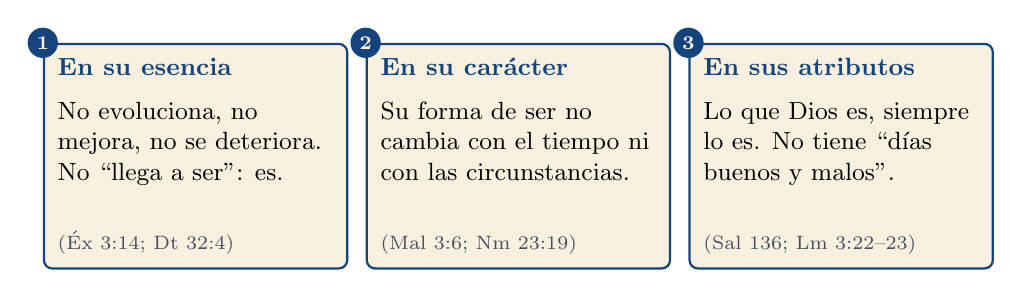
\begin{tikzpicture}
 \foreach \x/\n/\t/\d/\r in {0/1/{En su esencia}/{No evoluciona, no mejora, no se deteriora. No ``llega a ser'': es.}/{Éx 3:14; Dt 32:4},
   4.1/2/{En su carácter}/{Su forma de ser no cambia con el tiempo ni con las circunstancias.}/{Mal 3:6; Nm 23:19},
   8.2/3/{En sus atributos}/{Lo que Dios es, siempre lo es. No tiene ``días buenos y malos''.}/{Sal 136; Lm 3:22--23}}{
  \node[caja,anchor=north] (b\n) at (\x,0) {\parbox[t][2.5cm][t]{3.5cm}{\RaggedRight
    {\small\textbf{\textcolor{azul}{\t}}}\\[5pt]\small \d\par\vfill{\scriptsize\color{gris}(\r)}}};
  \node[circle,fill=azul,text=papiro,font=\scriptsize\bfseries,inner sep=1.6pt] at (b\n.north west) {\n};}
\end{tikzpicture}\par\medskip
\scriptsize\renewcommand{\arraystretch}{1.12}
\begin{tabular}{@{}>{\RaggedRight\arraybackslash}p{2.0cm}>{\RaggedRight\arraybackslash}p{3.0cm}>{\RaggedRight\arraybackslash}p{6.6cm}@{}}
\toprule
\textbf{Atributo} & \textbf{Texto} & \textbf{Lo que enseña} \\ \midrule
Misericordia & Sal 136 & ``Porque para siempre es su misericordia'' (\heb{כִּי לְעוֹלָם חַסְדּוֹ}) \\
Fidelidad & Lm 3:22--23 & ``Grande es tu fidelidad'' \\
Santidad & Is 6:3 & Dios no se vuelve menos santo \\
Verdad & Sal 119:89 & ``Para siempre\ldots{} permanece tu palabra en los cielos'' \\
\bottomrule
\end{tabular}
\end{frame}

\begin{frame}{Tu esquema y el de Pink}
\scriptsize\renewcommand{\arraystretch}{1.2}
\begin{tabular}{@{}>{\RaggedRight\arraybackslash}p{2.0cm}>{\RaggedRight\arraybackslash}p{4.6cm}>{\RaggedRight\arraybackslash}p{5.2cm}@{}}
\toprule
 & \textbf{Esta serie} & \textbf{Pink (2020, cap. 7)} \\ \midrule
1 & Inmutable en su \destacar{esencia} & ``inmutable en su esencia'': ``No hay arrugas en la frente de la eternidad'' \\
2 & Inmutable en su \destacar{carácter} & --- (lo incluye en esencia y atributos) \\
3 & Inmutable en sus \destacar{atributos} & ``inmutable en sus atributos'': \emph{Semper idem} \\
4 & --- (se trata en ``¿se arrepiente?'') & ``inmutable en su \destacar{consejo}'': ``Su voluntad nunca varía'' \\
\bottomrule
\end{tabular}\par\medskip
\begin{columns}[t,onlytextwidth]
\begin{column}{0.52\textwidth}\small
Pink argumenta: un hombre cambia de planes por falta de previsión o por falta de poder; Dios no tiene ninguna de las dos carencias, por eso ``nunca es necesario que revise sus decretos''.
\end{column}
\begin{column}{0.46\textwidth}
\precision{Pink se usa como referencia puntual. La diferencia de énfasis en el ``consejo'' se retoma en la sección sobre Jeremías 18.}
\end{column}
\end{columns}
\end{frame}

% ------------------------------------------------------------------
\section{¿Se arrepiente?}

\begin{frame}{``Pero la Biblia dice que Dios se arrepiente\ldots''}
\begin{columns}[t,onlytextwidth]
\begin{column}{0.50\textwidth}
\begin{cita}Y se arrepintió \SENOR{} de haber hecho hombre en la tierra, y le dolió en su corazón.\fuente{(Gn 6:6, RVR1960)}\end{cita}
\begin{cita}Entonces \SENOR{} se arrepintió del mal que dijo que había de hacer a su pueblo.\fuente{(Éx 32:14, RVR1960)}\end{cita}
\begin{cita}Y vio Dios lo que hicieron, que se convirtieron de su mal camino; y se arrepintió del mal que había dicho que les haría, y no lo hizo.\fuente{(Jon 3:10, RVR1960)}\end{cita}
\end{column}
\begin{column}{0.48\textwidth}
\begin{cita}Dios no es hombre, para que mienta, ni hijo de hombre para que se arrepienta. El dijo, ¿y no hará? Habló, ¿y no lo ejecutará?\fuente{(Nm 23:19, RVR1960)}\end{cita}
\small Los mismos libros dicen que Dios ``se arrepiente'' y que ``no se arrepiente''. Aquí entra la riqueza del pensamiento hebreo.
\end{column}
\end{columns}
\end{frame}

\begin{frame}{\emph{Najam}: el campo de la palabra}
\begin{columns}[c,onlytextwidth]
\begin{column}{0.52\textwidth}
\centering
\begin{tikzpicture}[font=\scriptsize]
 \node[draw=dorado,line width=1.6pt,fill=azul,text=papiro,circle,minimum size=1.4cm,align=center] (c) at (0,0) {\heb{נחם}\\ \emph{najam}};
 \foreach \a/\t/\r in {90/{consolar, consolarse}/{Gn 24:67; Is 40:1},
   18/{compadecerse}/{Jue 21:15; Sal 135:14},
   -54/{lamentar, ``me pesa''}/{1 S 15:11},
   -126/{desistir, cambiar de curso}/{Éx 32:14; Jon 3:10},
   162/{aplacarse, satisfacerse}/{Is 1:24; Ez 5:13}}{
  \node[caja,text width=2.0cm,align=center] (n\a) at (\a:2.5cm) {\t\\ {\tiny\color{gris}\r}};
  \draw[dorado,line width=1pt] (c)--(n\a);}
\end{tikzpicture}
\end{column}
\begin{column}{0.46\textwidth}\small
\begin{itemize}
\item \heb{נחם} \emph{najam} = lamentarse, compadecerse, \destacar{cambiar de curso de acción}.
\item Con Dios como sujeto describe casi siempre un \destacar{cambio de trato}: deja de hacer el mal anunciado (o el bien prometido).
\item Nunca dice que Dios reconozca un \destacar{error}: no hay confesión de pecado en Dios.
\end{itemize}
\end{column}
\end{columns}
\end{frame}

\begin{frame}{Dios y \emph{najam} en el AT}
\scriptsize\renewcommand{\arraystretch}{1.16}
\begin{tabular}{@{}>{\RaggedRight\arraybackslash}p{2.6cm}>{\RaggedRight\arraybackslash}p{0.7cm}>{\RaggedRight\arraybackslash}p{8.5cm}@{}}
\toprule
\textbf{Uso} & \textbf{vv.} & \textbf{Textos} \\ \midrule
Dios desiste, se lamenta o se compadece & 20 & Gn 6:6, 7; Éx 32:14; Dt 32:36; Jue 2:18; 1 S 15:11, 35; 2 S 24:16; 1 Cr 21:15; Sal 106:45; 135:14; Jer 18:8, 10; 26:3, 13, 19; 42:10; Am 7:3, 6; Jon 3:10 \\
Parte de la fórmula del carácter & 2 & ``y que se duele del castigo'' (Jl 2:13); ``y que te arrepientes del mal'' (Jon 4:2) \\
Se le pide o se espera & 4 & Éx 32:12; Sal 90:13; Jl 2:14; Jon 3:9 \\
Se niega que Dios lo haga & 8 & Nm 23:19; 1 S 15:29; Sal 110:4; Jer 4:28; 15:6; 20:16; Ez 24:14; Zac 8:14 \\
\bottomrule
\end{tabular}\par\medskip
\begin{columns}[t,onlytextwidth]
\begin{column}{0.52\textwidth}\small
Las negaciones tienen un patrón: Dios \destacar{juró} (Sal 110:4), \destacar{habló} (Nm 23:19; Ez 24:14) o ya \destacar{decidió} un juicio después de mucha paciencia (Jer 15:6: ``estoy cansado de arrepentirme'').
\end{column}
\begin{column}{0.46\textwidth}
\precision{conteo propio por raíz consonántica en la BHS, con Dios como sujeto (unos 34 versículos); verificar en e-Sword. La clasificación de cada texto es propia.}
\end{column}
\end{columns}
\end{frame}

\begin{frame}{Génesis 6:6: lo que leyeron las versiones}
\begin{center}\heb{וַיִּנָּחֶם יְהוָה כִּי־עָשָׂה אֶת־הָאָדָם בָּאָרֶץ וַיִּתְעַצֵּב אֶל־לִבּוֹ}\end{center}
\scriptsize\renewcommand{\arraystretch}{1.2}
\begin{tabular}{@{}>{\RaggedRight\arraybackslash}p{2.3cm}>{\RaggedRight\arraybackslash}p{5.3cm}>{\RaggedRight\arraybackslash}p{4.2cm}@{}}
\toprule
\textbf{Testigo} & \textbf{Texto} & \textbf{Sentido} \\ \midrule
TM & \heb{וַיִּנָּחֶם}\ldots{} \heb{וַיִּתְעַצֵּב אֶל־לִבּוֹ} & ``se lamentó\ldots{} y le dolió en su corazón'' \\
LXX 6:6 & \grc{καὶ ἐνεθυμήθη ὁ θεὸς\ldots{} καὶ διενοήθη} & ``y Dios lo tomó a pecho\ldots{} y lo consideró'' \\
LXX 6:7 & \grc{ὅτι ἐθυμώθην ὅτι ἐποίησα αὐτούς} & ``porque me he airado por haberlos hecho'' \\
Ónkelos & \heb{וְתָב יְיָ בְּמֵימְרֵהּ} & ``y el \SENOR{} volvió (se arrepintió) en su Palabra'' \\
\bottomrule
\end{tabular}\par\medskip
\begin{columns}[t,onlytextwidth]
\begin{column}{0.52\textwidth}\small
El texto hebreo no suaviza: habla del \destacar{dolor} de Dios (\heb{עצב}, la misma raíz del ``dolor'' de Gn 3:16--17). La LXX ya evita decir que Dios se arrepintió.
\end{column}
\begin{column}{0.46\textwidth}
\precision{(textual) la LXX traduce \emph{najam} de Gn 6:6 por \grc{ἐνθυμέομαι} y en Éx 32:14 por \grc{ἱλάσκομαι} (``se aplacó''); en Jon 3:10 y Jer 18:8 sí usa \grc{μετανοέω}.}
\end{column}
\end{columns}
\end{frame}

\begin{frame}{1 Samuel 15: las dos cosas en un capítulo}
\begin{columns}[t,onlytextwidth]
\begin{column}{0.50\textwidth}
\begin{cita}Me pesa haber puesto por rey a Saúl, porque se ha vuelto de en pos de mí, y no ha cumplido mis palabras.\fuente{(1 S 15:11, RVR1960)}\end{cita}
\begin{cita}Además, el que es la Gloria de Israel no mentirá, ni se arrepentirá, porque no es hombre para que se arrepienta.\fuente{(1 S 15:29, RVR1960)}\end{cita}
\begin{cita}\ldots{} y \SENOR{} se arrepentía de haber puesto a Saúl por rey sobre Israel.\fuente{(1 S 15:35, RVR1960)}\end{cita}
\end{column}
\begin{column}{0.48\textwidth}\small
\begin{itemize}
\item v. 11 y 35: \heb{נִחַמְתִּי}, \heb{נִחָם}: Dios \destacar{lamenta} lo ocurrido con Saúl.
\item v. 29: \heb{וְלֹא יִנָּחֵם}: Dios no \destacar{revoca} la sentencia ya dada.
\item \heb{נֵצַח יִשְׂרָאֵל} \emph{nétsaj Yisra'el}: ``la Gloria / el Eterno / la Victoria de Israel'' (\emph{nétsaj}: perpetuidad, preeminencia).
\item El narrador pone las dos afirmaciones a pocos versos: \destacar{no ve contradicción}.
\end{itemize}
\end{column}
\end{columns}\par\smallskip
\precision{Rashi (1 S 15:29): aunque Saúl diga ``me arrepentiré'', ya no servirá para quitar el reino a quien Dios se lo dio, porque el \emph{Nétsaj} de Israel ``no mentirá'' dejando de dar el bien que dijo que daría.}
\end{frame}

\begin{frame}{``Y que te arrepientes del mal''}
\begin{columns}[t,onlytextwidth]
\begin{column}{0.52\textwidth}
\begin{cita}\ldots{} porque sabía yo que tú eres Dios clemente y piadoso, tardo en enojarte, y de grande misericordia, y que te arrepientes del mal.\fuente{(Jon 4:2, RVR1960)}\end{cita}
\begin{center}\heb{כִּי אַתָּה אֵל־חַנּוּן וְרַחוּם}\\[2pt]\heb{אֶרֶךְ אַפַּיִם וְרַב־חֶסֶד וְנִחָם עַל־הָרָעָה}\end{center}
\end{column}
\begin{column}{0.46\textwidth}\small
\begin{itemize}
\item Jonás y Joel (2:13) citan el Nombre de Éx 34:6 y le añaden \heb{וְנִחָם עַל־הָרָעָה}: ``y que desiste del mal''.
\item El ``arrepentirse'' de Dios no contradice su carácter: \destacar{forma parte} de su carácter revelado.
\item Dios desiste del juicio \destacar{porque} no cambia: porque es siempre clemente y piadoso.
\end{itemize}
\end{column}
\end{columns}\par\smallskip
\begin{tcolorbox}[colback=papiro,colframe=dorado,boxrule=1.2pt,arc=3pt]
\small Estos textos no muestran un Dios que cometió un error, sino un Dios que \destacar{responde moralmente}.
\end{tcolorbox}
\end{frame}

\begin{frame}{``Porque Dios soy, y no hombre''}
\begin{columns}[t,onlytextwidth]
\begin{column}{0.50\textwidth}
\begin{cita}¿Cómo podré abandonarte, oh Efraín?\ldots{} Mi corazón se conmueve dentro de mí, se inflama toda mi compasión. No ejecutaré el ardor de mi ira, ni volveré para destruir a Efraín; porque Dios soy, y no hombre, el Santo en medio de ti.\fuente{(Os 11:8--9, RVR1960)}\end{cita}
\end{column}
\begin{column}{0.48\textwidth}
\scriptsize\renewcommand{\arraystretch}{1.18}
\begin{tabular}{@{}>{\RaggedRight\arraybackslash}p{1.4cm}>{\RaggedRight\arraybackslash}p{3.8cm}@{}}
\toprule
\textbf{Texto} & \textbf{``No es hombre''\ldots} \\ \midrule
Nm 23:19 & \ldots{} ``para que se arrepienta'': no revoca su bendición. \\
1 S 15:29 & \ldots{} ``para que se arrepienta'': no revoca su juicio. \\
Os 11:9 & \ldots{} por eso \destacar{no destruye}: \heb{נִכְמְרוּ נִחוּמָי}, ``se inflama mi compasión'' (\emph{nijumay}, de \heb{נחם}). \\
\bottomrule
\end{tabular}\par\smallskip
\small Ser ``Dios y no hombre'' funda a la vez su firmeza y su compasión.
\end{column}
\end{columns}
\end{frame}

% ------------------------------------------------------------------
\section{Jeremías 18}

\begin{frame}{El alfarero (Jer 18:1--6)}
\begin{columns}[t,onlytextwidth]
\begin{column}{0.52\textwidth}
\begin{cita}Y descendí a casa del alfarero, y he aquí que él trabajaba sobre la rueda. Y la vasija de barro que él hacía se echó a perder en su mano; y volvió y la hizo otra vasija, según le pareció mejor hacerla\ldots{} ¿No podré yo hacer de vosotros como este alfarero, oh casa de Israel? dice \SENOR.\fuente{(Jer 18:3--6, RVR1960)}\end{cita}
\end{column}
\begin{column}{0.46\textwidth}\small
\begin{itemize}
\item \heb{הַיּוֹצֵר} \emph{hayyotser}: ``el que forma'', de \heb{יצר}, el verbo de Gn 2:7 (``formó al hombre'').
\item \heb{עַל־הָאָבְנָיִם}: ``sobre las dos piedras'', el torno de dos discos.
\item El barro no es tratado mecánicamente: la acción del alfarero \destacar{depende del estado del barro}.
\item Dios es soberano, pero su trato es \destacar{relacional y moral}, no fatalista.
\end{itemize}
\end{column}
\end{columns}
\end{frame}

\begin{frame}{La clave interpretativa (Jer 18:7--10)}
\begin{columns}[t,onlytextwidth]
\begin{column}{0.49\textwidth}
\begin{cita}En un instante hablaré contra pueblos y contra reinos, para arrancar, y derribar, y destruir. Pero si esos pueblos se convirtieren de su maldad contra la cual hablé, yo me arrepentiré del mal que había pensado hacerles,\fuente{(Jer 18:7--8, RVR1960)}\end{cita}
\begin{center}\heb{וְשָׁב הַגּוֹי הַהוּא מֵרָעָתוֹ}\ldots{} \heb{וְנִחַמְתִּי עַל־הָרָעָה}\end{center}
\end{column}
\begin{column}{0.49\textwidth}
\begin{cita}y en un instante hablaré de la gente y del reino, para edificar y para plantar. Pero si hiciere lo malo delante de mis ojos, no oyendo mi voz, me arrepentiré del bien que había determinado hacerle.\fuente{(Jer 18:9--10, RVR1960)}\end{cita}
\begin{center}\heb{וְנִחַמְתִּי עַל־הַטּוֹבָה}\end{center}
\end{column}
\end{columns}\par\smallskip
\small\RaggedRight Los verbos de 18:7 y 18:9 (``arrancar, derribar, destruir''; ``edificar, plantar'') son los del llamamiento de Jeremías (Jer 1:10).
\end{frame}

\begin{frame}{Un gobierno condicional}
\centering
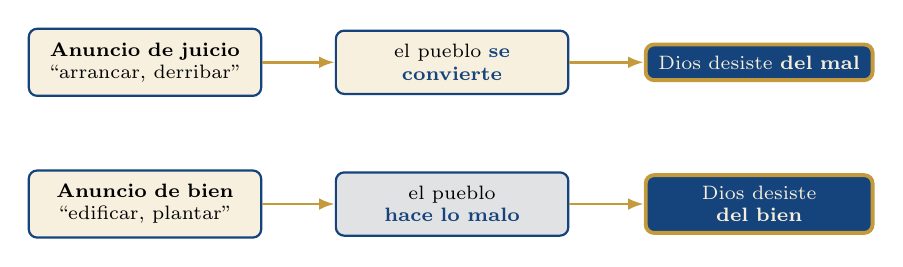
\begin{tikzpicture}[font=\scriptsize]
 \node[caja,text width=2.6cm,align=center] (a) at (0,1.2) {\textbf{Anuncio de juicio}\\ ``arrancar, derribar''};
 \node[caja,text width=2.6cm,align=center] (b) at (0,-0.6) {\textbf{Anuncio de bien}\\ ``edificar, plantar''};
 \node[caja,text width=2.6cm,align=center] (c) at (3.9,1.2) {el pueblo \destacar{se convierte}};
 \node[caja,text width=2.6cm,align=center,fill=gris!18] (d) at (3.9,-0.6) {el pueblo \destacar{hace lo malo}};
 \node[draw=dorado,line width=1.4pt,fill=azul,text=papiro,rounded corners=3pt,text width=2.6cm,align=center,inner sep=4pt] (e) at (7.8,1.2) {Dios desiste \textbf{del mal}};
 \node[draw=dorado,line width=1.4pt,fill=azul,text=papiro,rounded corners=3pt,text width=2.6cm,align=center,inner sep=4pt] (f) at (7.8,-0.6) {Dios desiste \textbf{del bien}};
 \draw[-{Latex[length=2mm]},dorado,line width=1pt] (a)--(c); \draw[-{Latex[length=2mm]},dorado,line width=1pt] (c)--(e);
 \draw[-{Latex[length=2mm]},dorado,line width=1pt] (b)--(d); \draw[-{Latex[length=2mm]},dorado,line width=1pt] (d)--(f);
\end{tikzpicture}\par\medskip
\begin{tcolorbox}[colback=papiro,colframe=dorado,boxrule=1.2pt,arc=3pt]
\small \textbf{Principio revelado por Dios mismo:} las declaraciones divinas sobre juicio o bendición suelen ser \destacar{condicionales a la respuesta humana}.
\end{tcolorbox}
\small\RaggedRight Lo constante es el criterio: Dios trata siempre igual al que se vuelve y al que persiste en el mal. Por eso su ``arrepentirse'' es la forma visible de su \destacar{justicia inmutable}.\par\smallskip
\precision{la última frase es síntesis teológica de esta serie.}
\end{frame}

\begin{frame}{El pueblo cambia; Dios responde}
\begin{columns}[t,onlytextwidth]
\begin{column}{0.50\textwidth}\small
\begin{itemize}
\item En Jer 18:8 el que \destacar{vuelve} primero es el pueblo: \heb{וְשָׁב הַגּוֹי} (\emph{veshav hagoy}). Dios responde: \heb{וְנִחַמְתִּי}.
\item Lo que cambia es la \destacar{relación} del pueblo con Dios; Dios aplica a la nueva situación el mismo carácter de siempre.
\item Jer 18:11 es una invitación: ``conviértase ahora cada uno de su mal camino''.
\end{itemize}
\end{column}
\begin{column}{0.48\textwidth}
\begin{cita}Y dijeron: Es en vano; porque en pos de nuestros ídolos iremos, y haremos cada uno el pensamiento de nuestro malvado corazón.\fuente{(Jer 18:12, RVR1960)}\end{cita}
\small Judá rechaza la oferta. La condición estaba abierta; la puerta la cerró el pueblo, no Dios.
\end{column}
\end{columns}\par\smallskip
\precision{el texto masorético de 18:12 dice ``en pos de nuestros pensamientos'' (\heb{אַחֲרֵי מַחְשְׁבוֹתֵינוּ}); la RVR1960 traduce ``ídolos''.}
\end{frame}

\begin{frame}{Dos ejemplos: Nínive y Ezequías}
\begin{columns}[t,onlytextwidth]
\begin{column}{0.49\textwidth}
\begin{cita}Ordena tu casa, porque morirás, y no vivirás\ldots{} He oído tu oración, y visto tus lágrimas; he aquí que yo añado a tus días quince años.\fuente{(Is 38:1, 5, RVR1960)}\end{cita}
\scriptsize El anuncio a Ezequías no era un decreto ciego: la oración era el \destacar{medio} que Dios había dispuesto para obrar. La señal fue la sombra que retrocedió en el reloj de Acaz (38:8).
\end{column}
\begin{column}{0.49\textwidth}
\begin{cita}De aquí a cuarenta días Nínive será destruida.\fuente{(Jon 3:4, RVR1960)}\end{cita}
\scriptsize Jonás anuncia un juicio sin condiciones explícitas. El rey responde: ``¿Quién sabe si se volverá y se arrepentirá Dios\ldots?'' (3:9). Y Dios desiste (3:10). Jer 18:7--8 explica el caso.\par\smallskip
Los ancianos de Judá recuerdan lo mismo de Ezequías ante Miqueas: ``¿No temió\ldots{} y oró\ldots{} y \SENOR{} se arrepintió?'' (Jer 26:19).
\end{column}
\end{columns}
\end{frame}

\begin{frame}{¿Decreto fijo o anuncio condicional?}
\scriptsize\renewcommand{\arraystretch}{1.2}
\begin{tabular}{@{}>{\RaggedRight\arraybackslash}p{2.3cm}>{\RaggedRight\arraybackslash}p{4.7cm}>{\RaggedRight\arraybackslash}p{4.8cm}@{}}
\toprule
 & \textbf{Lo que nunca cambia} & \textbf{Lo que responde} \\ \midrule
Texto & ``El consejo de \SENOR{} permanecerá para siempre'' (Sal 33:11); ``Mi consejo permanecerá'' (Is 46:10) & ``me arrepentiré del mal\ldots{} me arrepentiré del bien'' (Jer 18:8, 10) \\
Objeto & el propósito, el pacto, lo jurado & los anuncios de juicio o de bendición en la historia \\
Pink & ``Su voluntad nunca varía''; el ``arrepentirse'' describe ``un cambio en sus tratos'' & ``Cuando Él instituye un cambio en sus tratos con los hombres\ldots'' \\
Tu material & Dios no cambia en naturaleza, carácter, santidad y fidelidad & Dios sí cambia en su trato histórico, en la aplicación de juicio o misericordia y en su respuesta a la oración \\
\bottomrule
\end{tabular}\par\medskip
\small\RaggedRight Pink y tu material coinciden en algo central: lo que la Biblia llama ``arrepentirse'' en Dios es un \destacar{cambio de trato}, no de ser.\par\smallskip
\precision{difieren en el énfasis: Pink lo explica como lenguaje adaptado a nosotros (``adapta su lenguaje a nuestras capacidades limitadas''); tu material lo lee como un cambio real en la relación histórica. Las dos lecturas tienen defensores.}
\end{frame}

% ------------------------------------------------------------------
\section{¿Cambia o no?}

\begin{frame}{Entonces, ¿Dios cambia o no?}
\begin{columns}[t,onlytextwidth]
\begin{column}{0.48\textwidth}
\begin{tcolorbox}[colback=papiro,colframe=azul,boxrule=1pt,arc=3pt,title={\small Dios NO cambia en},colbacktitle=azul,coltitle=papiro]
\small
\begin{itemize}
\item su naturaleza (Éx 3:14; Sal 102:27);
\item su carácter (Mal 3:6; Jon 4:2);
\item su santidad (Is 6:3);
\item su fidelidad al pacto (Sal 89:34; Lm 3:23).
\end{itemize}
\end{tcolorbox}
\end{column}
\begin{column}{0.48\textwidth}
\begin{tcolorbox}[colback=papiro,colframe=dorado,boxrule=1pt,arc=3pt,title={\small Dios SÍ cambia en},colbacktitle=dorado,coltitle=azuloscuro]
\small
\begin{itemize}
\item su trato histórico (1 S 15:11);
\item la aplicación de juicio o misericordia (Jer 18:7--10);
\item su respuesta a la oración y al arrepentimiento (Éx 32:14; Is 38:5; Jon 3:10).
\end{itemize}
\end{tcolorbox}
\end{column}
\end{columns}\par\medskip
\centering\destacar{Esto no es contradicción: es coherencia viva.}
\end{frame}

\begin{frame}{Definición}
\begin{tcolorbox}[colback=papiro,colframe=azul,boxrule=1pt,arc=3pt,title={\small Definición teológica bíblica},colbacktitle=azul,coltitle=papiro]
\small La inmutabilidad de Dios significa que Él es eternamente el mismo en su ser y carácter, pero su gobierno del mundo es dinámico y responde de manera coherente a la conducta humana.
\end{tcolorbox}
\scriptsize\renewcommand{\arraystretch}{1.18}
\begin{tabular}{@{}>{\RaggedRight\arraybackslash}p{3.0cm}>{\RaggedRight\arraybackslash}p{8.8cm}@{}}
\toprule
\textbf{Elemento} & \textbf{Texto que lo funda} \\ \midrule
``eternamente el mismo'' & ``pero tú eres el mismo, y tus años no se acabarán'' (Sal 102:27) \\
``en su ser y carácter'' & ``Porque yo \SENOR{} no cambio'' (Mal 3:6); ``YO SOY EL QUE SOY'' (Éx 3:14) \\
``gobierno dinámico'' & ``¿No podré yo hacer de vosotros como este alfarero?'' (Jer 18:6) \\
``responde de manera coherente'' & ``Volveos a mí, y yo me volveré a vosotros'' (Mal 3:7); ``y que te arrepientes del mal'' (Jon 4:2) \\
\bottomrule
\end{tabular}
\end{frame}

\begin{frame}{Dos maneras de pensar la inmutabilidad}
\scriptsize\renewcommand{\arraystretch}{1.13}
\begin{tabular}{@{}>{\RaggedRight\arraybackslash}p{2.3cm}>{\RaggedRight\arraybackslash}p{4.5cm}>{\RaggedRight\arraybackslash}p{5.0cm}@{}}
\toprule
\textbf{Aspecto} & \textbf{Inmutabilidad filosófica (griega)} & \textbf{Inmutabilidad bíblica hebrea} \\ \midrule
Cambio & Todo cambio implica imperfección & Cambio relacional no afecta la perfección \\
Emociones divinas & No son reales & Son expresiones verdaderas del carácter \\
Respuesta a humanos & Dios no ``reacciona'' & Dios responde moralmente \\
Decretos & Absolutamente fijos e incondicionales & Muchos anuncios son condicionales (Jer 18:7--10) \\
Arrepentimiento divino & Solo figura literaria & Cambio real de trato histórico \\
Relación con la oración & No altera nada & Medio establecido por Dios para obrar (Éx 32; Is 38) \\
Enfoque principal & Inmutabilidad = inmovilidad & Inmutabilidad = fidelidad coherente \\
\bottomrule
\end{tabular}\par\smallskip
\precision{la tabla contrasta énfasis. La columna izquierda reúne ideas de Platón y de la filosofía griega, pero también posiciones de autores judíos y cristianos (Filón, Maimónides, la teología clásica, Pink), que afirman la realidad del amor y de la respuesta de Dios aunque lean ``arrepentirse'' como lenguaje adaptado. Ver la lámina siguiente.}
\end{frame}

\begin{frame}{De dónde viene la columna ``filosófica''}
\scriptsize\renewcommand{\arraystretch}{1.18}
\begin{tabular}{@{}>{\RaggedRight\arraybackslash}p{2.6cm}>{\RaggedRight\arraybackslash}p{9.2cm}@{}}
\toprule
\textbf{Platón} (\emph{República} II, 381c) & ``Es imposible, entonces, que un dios quiera alterarse a sí mismo; cada uno, siendo lo más bello y lo mejor posible, permanece siempre simplemente en su propia forma''. Si es perfecto, cualquier cambio sería a peor. \\
\textbf{Filón} (\emph{Quod Deus} 52--54) & Judío de Alejandría. Comenta Gn 6:6 y dice que Dios no está sujeto a pasiones; la Torá tiene dos principios: ``Dios no es como hombre'' (Nm 23:19), que es la verdad, y ``como un hombre\ldots{} a su hijo'' (Dt 1:31), dicho ``para instrucción'' de los muchos. \\
\textbf{Maimónides} (\emph{Yesodé haTorá} 1:11--12) & ``No cambia, porque no hay nada que le cause cambio''. La ira y la alegría de Dios en la Biblia son ``metáfora'': ``la Torá habla en lenguaje de los hombres''. Y cita Mal 3:6: ``si a veces se enojara y a veces se alegrara, cambiaría''. \\
\textbf{Pink} (2020, cap. 7) & ``Cuando habla de Sí mismo, Dios, con frecuencia, adapta su lenguaje a nuestras capacidades limitadas''. \\
\bottomrule
\end{tabular}\par\medskip
\small\RaggedRight La lectura ``filosófica'' no es solo griega: entró en el judaísmo y en el cristianismo. La mirada hebrea de tu material deja que el texto diga las dos cosas: Dios es el mismo (Mal 3:6) y Dios \destacar{siente y responde} (Gn 6:6; Os 11:8).\par\smallskip
\precision{Platón según la trad. de Shorey (1930); Filón según la de Yonge (1854); Maimónides según Sefaria. Traducción al español propia.}
\end{frame}

% ------------------------------------------------------------------
\section{En Israel}

\begin{frame}{Balaam: maldecir a sueldo}
\centering
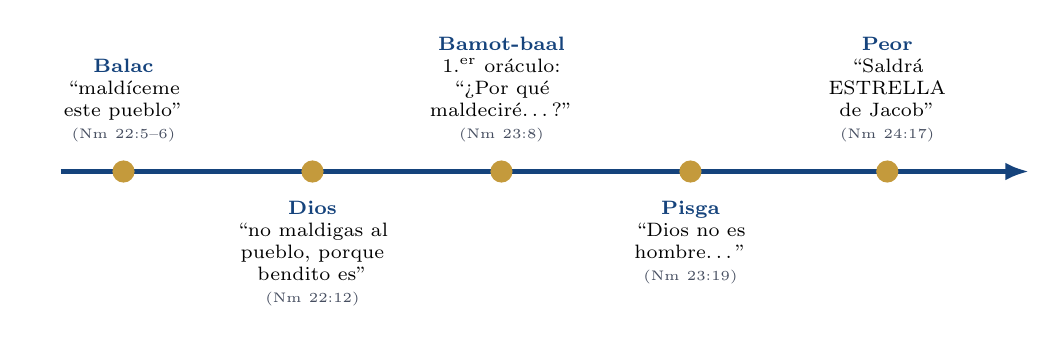
\begin{tikzpicture}[font=\scriptsize]
 \draw[line width=1.6pt,azul,-{Latex[length=3mm]}] (-0.3,0) -- (12.0,0);
 \foreach \x/\t/\b/\r/\pos in {0.5/{Balac}/{``maldíceme este pueblo''}/{Nm 22:5--6}/above,
   2.9/{Dios}/{``no maldigas al pueblo, porque bendito es''}/{Nm 22:12}/below,
   5.3/{Bamot-baal}/{1.\textsuperscript{er} oráculo: ``¿Por qué maldeciré\ldots?''}/{Nm 23:8}/above,
   7.7/{Pisga}/{``Dios no es hombre\ldots''}/{Nm 23:19}/below,
   10.2/{Peor}/{``Saldrá ESTRELLA de Jacob''}/{Nm 24:17}/above}{
  \fill[dorado] (\x,0) circle (4pt);
  \node[\pos=7pt,text width=2.2cm,align=center] at (\x,0) {\textbf{\textcolor{azul}{\t}}\\ \b\\ {\tiny\color{gris}(\r)}};}
\end{tikzpicture}\par\medskip
\begin{columns}[t,onlytextwidth]
\begin{column}{0.49\textwidth}
\begin{cita}Te ruego que vengas conmigo a otro lugar desde el cual los veas\ldots{} y desde allí me los maldecirás.\fuente{(Nm 23:13, RVR1960)}\end{cita}
\end{column}
\begin{column}{0.49\textwidth}\small
Balac cambia de \destacar{lugar} tres veces, cambia de \destacar{altares} (siete toros y siete carneros cada vez) y espera que Dios cambie de \destacar{palabra}: ``por ventura parecerá bien a Dios que desde allí me lo maldigas'' (23:27).
\end{column}
\end{columns}
\end{frame}

\begin{frame}{``Dios no es hombre''}
\fotolado{panel_numeros23.jpg}{Elaboración propia: Nm 23:19 en texto hebreo consonántico (BHS).}
\begin{columns}[c,onlytextwidth]
\begin{column}{0.58\textwidth}
\begin{cita}Dios no es hombre, para que mienta, ni hijo de hombre para que se arrepienta. El dijo, ¿y no hará? Habló, ¿y no lo ejecutará? He aquí, he recibido orden de bendecir; El dio bendición, y no podré revocarla.\fuente{(Nm 23:19--20, RVR1960)}\end{cita}
\small Lo dice un adivino pagano contratado para maldecir. La inmutabilidad de Dios aparece aquí como \destacar{protección del pueblo}: la bendición dada a Israel no se compra ni se revoca.
\end{column}
\begin{column}{0.40\textwidth}\end{column}
\end{columns}
\end{frame}

\begin{frame}{Nm 23:19--20 en hebreo}
\begin{center}\heb{לֹא אִישׁ אֵל וִיכַזֵּב וּבֶן־אָדָם וְיִתְנֶחָם}\\[2pt]\heb{הַהוּא אָמַר וְלֹא יַעֲשֶׂה וְדִבֶּר וְלֹא יְקִימֶנָּה}\end{center}
\scriptsize\renewcommand{\arraystretch}{1.13}
\begin{tabular}{@{}>{\RaggedRight\arraybackslash}p{2.9cm}>{\RaggedRight\arraybackslash}p{1.1cm}>{\RaggedRight\arraybackslash}p{7.9cm}@{}}
\toprule
\textbf{Término} & \textbf{Raíz} & \textbf{Sentido} \\ \midrule
\heb{לֹא אִישׁ אֵל} & --- & ``no (es) hombre Dios'': frase nominal, sin verbo; el contraste es de naturaleza. \\
\heb{וִיכַזֵּב} \emph{vijazzev} & \heb{כזב} & ``para que mienta'': \emph{kazav}, la palabra que falla, como el arroyo que se seca (Is 58:11). \\
\heb{וְיִתְנֶחָם} \emph{veyitneján} & \heb{נחם} & ``para que se arrepienta'': hitpael, ``cambiar de parecer''. \\
\heb{וְלֹא יְקִימֶנָּה} & \heb{קום} & ``¿y no la hará estar en pie?'': su palabra se levanta y se mantiene. \\
\heb{וְלֹא אֲשִׁיבֶנָּה} (v. 20) & \heb{שׁוב} & ``y no la haré volver'': ``no podré revocarla''. \\
\bottomrule
\end{tabular}\par\medskip
\small\textbf{LXX:} \grc{οὐχ ὡς ἄνθρωπος ὁ θεὸς διαρτηθῆναι οὐδὲ ὡς υἱὸς ἀνθρώπου ἀπειληθῆναι}: ``Dios no es como hombre para vacilar, ni como hijo de hombre para ser amenazado''.\par\smallskip
\precision{(textual) la LXX interpreta libremente la primera línea; sigue el sentido general, no las palabras del TM.}
\end{frame}

\begin{frame}{La maldición convertida en bendición}
\begin{columns}[t,onlytextwidth]
\begin{column}{0.50\textwidth}
\begin{cita}Mas no quiso \SENOR{} tu Dios oír a Balaam; y \SENOR{} tu Dios te convirtió la maldición en bendición, porque \SENOR{} tu Dios te amaba.\fuente{(Dt 23:5 [23:6], RVR1960)}\end{cita}
\begin{center}\heb{וַיַּהֲפֹךְ יְהוָה אֱלֹהֶיךָ לְּךָ אֶת־הַקְּלָלָה לִבְרָכָה}\end{center}
\end{column}
\begin{column}{0.48\textwidth}\small
\begin{itemize}
\item Lo que Dios ``da vuelta'' (\heb{הפך} \emph{hafaj}) es la \destacar{maldición}, no su palabra.
\item La causa: ``porque te amaba'' (\heb{כִּי אֲהֵבְךָ}). La inmutabilidad es la de un \destacar{amor} de pacto.
\item Nehemías lo recuerda siglos después: ``mas nuestro Dios volvió la maldición en bendición'' (Neh 13:2).
\item Miqueas manda recordar a Balac y a Balaam ``para que conozcas las justicias de \SENOR'' (Mi 6:5).
\end{itemize}
\end{column}
\end{columns}
\end{frame}

\begin{frame}{Lo que enseña el encuentro}
\begin{columns}[t,onlytextwidth]
\begin{column}{0.50\textwidth}
\scriptsize\renewcommand{\arraystretch}{1.2}
\begin{tabular}{@{}>{\RaggedRight\arraybackslash}p{2.4cm}>{\RaggedRight\arraybackslash}p{3.3cm}@{}}
\toprule
\textbf{El hombre cambia} & \textbf{Dios permanece} \\ \midrule
Balac cambia de lugar (23:13, 27) & ``El dio bendición'' (23:20) \\
Balac cambia de altares (23:1, 14, 29) & ``¿Por qué maldeciré yo al que Dios no maldijo?'' (23:8) \\
Balaam quiere el pago (2 P 2:15) & ``harás lo que yo te diga'' (22:20) \\
Israel cae en Baal-peor (25:1--3) & la promesa sigue: ``Saldrá ESTRELLA de Jacob'' (24:17) \\
\bottomrule
\end{tabular}
\end{column}
\begin{column}{0.48\textwidth}\small
\begin{itemize}
\item Rashi (Nm 23:19): Dios ya juró llevar a Israel a la tierra, ``¿y tú piensas matarlos en el desierto?''.
\item El oráculo dice ``No ha notado iniquidad en Jacob'' (23:21), y en el capítulo siguiente Israel peca en Baal-peor. La bendición no dependía de que Israel lo mereciera.
\end{itemize}
\precision{la lectura de Nm 25 como contraste con la bendición inmutable es lectura propia.}
\end{column}
\end{columns}
\end{frame}

% ------------------------------------------------------------------
\section{Judaísmo}

\begin{frame}{En la oración diaria}
\begin{columns}[t,onlytextwidth]
\begin{column}{0.50\textwidth}\small
\textbf{Bendiciones de la mañana} (\emph{Sidur}, Shajarit):
\begin{center}\heb{אַתָּה הוּא עַד שֶׁלֹּא נִבְרָא הָעוֹלָם}\\ \heb{אַתָּה הוּא מִשֶּׁנִּבְרָא הָעוֹלָם}\\ \heb{אַתָּה הוּא בָּעוֹלָם הַזֶּה}\\ \heb{וְאַתָּה הוּא לָעוֹלָם הַבָּא}\end{center}
``Tú eres él antes que el mundo fuera creado; tú eres él desde que el mundo fue creado; tú eres él en este mundo, y tú eres él en el mundo venidero''.
\end{column}
\begin{column}{0.48\textwidth}\small
\textbf{\emph{Adón olam}} (himno de la sinagoga):
\begin{center}\heb{וְהוּא הָיָה וְהוּא הֹוֶה}\\ \heb{וְהוּא יִהְיֶה בְּתִפְאָרָה}\end{center}
``Él fue, él es, y él será en gloria''.
\begin{center}\heb{בְּלִי רֵאשִׁית בְּלִי תַכְלִית}\end{center}
``Sin principio, sin fin''.
\end{column}
\end{columns}\par\smallskip
\precision{textos litúrgicos según el \emph{Sidur Ashkenaz} (Sefaria); el ``\emph{atá hu}'' retoma Sal 102:27. Traducción propia.}
\end{frame}

\begin{frame}{``Estaré con ellos'': Rashi y el Nombre}
\begin{columns}[t,onlytextwidth]
\begin{column}{0.52\textwidth}\small
\textbf{Rashi} a Éx 3:14, a partir de \emph{Berajot} 9b:
\begin{center}\heb{אֶהְיֶה עִמָּם בְּצָרָה זוֹ}\\ \heb{אֲשֶׁר אֶהְיֶה עִמָּם בְּשִׁעְבּוּד שְׁאָר מַלְכֻיּוֹת}\end{center}
``Estaré con ellos en esta angustia, el que estaré con ellos en la servidumbre de los otros reinos''.\par\smallskip
Moisés objeta: ``¿por qué recordarles otra angustia? Les basta con esta''. Dios le da la razón: ``Así dirás: \emph{Ehyé} me envió''.
\end{column}
\begin{column}{0.46\textwidth}
\begin{tcolorbox}[colback=papiro,colframe=dorado,boxrule=1.2pt,arc=3pt]
\small Para la tradición judía, el Nombre no describe un ser inmóvil, sino una \destacar{presencia fiel}: el mismo Dios en Egipto, en Babilonia y en cada exilio.
\end{tcolorbox}
\precision{interpretación rabínica (Sefaria: Rashi, trad. Rosenbaum y Silbermann; \emph{Berajot} 9b, ed. William Davidson). Traducción propia.}
\end{column}
\end{columns}
\end{frame}

\begin{frame}{Los targumes: ``no como los hombres''}
\scriptsize\renewcommand{\arraystretch}{1.2}
\begin{tabular}{@{}>{\RaggedRight\arraybackslash}p{2.4cm}>{\RaggedRight\arraybackslash}p{9.4cm}@{}}
\toprule
\textbf{Ónkelos} (Nm 23:19) & \heb{לָא כְמִלֵּי בְנֵי אֱנָשָׁא מֵימַר אֱלָהָא}\ldots{} \heb{דִּי אִנּוּן גָּזְרִין לְמֶעְבַּד וְתַיְּבִין וּמִתְמַלְּכִין}\par ``No como las palabras de los hombres es la Palabra de Dios; los hombres dicen y mienten\ldots{} deciden hacer, y se vuelven atrás y cambian de consejo. Él dice y hace, y toda su Palabra se cumple''. \\
\textbf{Targum Jonatán} (1 S 15:29) & \heb{וְלָא תָאִיב מִמָה דַאֲמַר אֲרֵי לָא כִּבְנֵי אֱנָשָׁא הוּא דְאָמְרִין וּמְכַדְבִין גָזְרִין וְלָא מְקַיְמִין}\par ``Y no se vuelve de lo que dijo, porque no es como los hijos de los hombres, que dicen y desmienten, deciden y no cumplen''. \\
\textbf{Ónkelos} (Gn 6:6) & \heb{וְתַב יְיָ בְּמֵימְרֵהּ}: ``y el \SENOR{} se volvió en su Palabra'': conserva el cambio, pero lo pone en la \emph{Memrá}. \\
\bottomrule
\end{tabular}\par\medskip
\small\RaggedRight Los targumes leen ``no se arrepiente'' como \destacar{fidelidad a la palabra dada}: lo que Dios dice, lo cumple.\par\smallskip
\precision{traducciones antiguas e interpretativas (Sefaria). Traducción propia.}
\end{frame}

\begin{frame}{Rashi y el Midrash sobre Gn 6:6}
\begin{columns}[t,onlytextwidth]
\begin{column}{0.50\textwidth}\scriptsize
\textbf{Rashi:}\par\begin{center}\heb{נֶהְפְּכָה מַחְשַׁבְתּוֹ שֶׁל מָקוֹם}\\ \heb{מִמִּדַּת רַחֲמִים לְמִדַּת הַדִּין}\end{center}``el pensamiento del Omnipresente se volvió de la medida de misericordia a la medida de justicia''.\par\smallskip
``Y así todo \emph{nijum} en la Escritura es lenguaje de \emph{nimlaj ma la'asot}, \destacar{deliberar qué hacer}'' (cita Nm 23:19; Dt 32:36; Éx 32:14; 1 S 15:11).
\end{column}
\begin{column}{0.48\textwidth}\scriptsize
\textbf{\emph{Bereshit Rabá} 27:4:} un hereje pregunta a Rabí Yehoshúa ben Qorjá: ``¿No dicen ustedes que Dios ve el futuro? ¿Y cómo dice que le dolió?''. El rabino responde: ``¿Te nació un hijo varón? ¿Qué hiciste?''. ``Me alegré e hice alegrar a todos''. ``¿Y no sabías que al final moriría?''. ``En la hora de la alegría, alegría; en la hora del duelo, duelo''.\par\smallskip
Rashi concluye: aunque estaba revelado ante él que pecarían, ``no se abstuvo de crearlos, por causa de los justos que habrían de salir de ellos''.
\end{column}
\end{columns}\par\medskip
\small\RaggedRight El Midrash no niega el dolor de Dios: lo une a su \destacar{presciencia}. Dios sabe y aun así ama, crea y se duele.\par\smallskip
\precision{interpretación rabínica (Sefaria). Traducción propia.}
\end{frame}

\begin{frame}{El decreto se rompe; Dios no cambia}
\begin{columns}[t,onlytextwidth]
\begin{column}{0.52\textwidth}\scriptsize
\textbf{\emph{Rosh Hashaná} 16b} (Rabí Yitsjaq):\par\begin{center}\heb{אַרְבָּעָה דְּבָרִים מְקָרְעִין גְּזַר דִּינוֹ שֶׁל אָדָם}\end{center}``Cuatro cosas rasgan el decreto contra una persona: la caridad, el clamor, el cambio de nombre y el \destacar{cambio de conducta}'' (\heb{שִׁינּוּי מַעֲשֶׂה}). Prueba: ``Y vio Dios sus obras\ldots{} y se arrepintió del mal'' (Jon 3:10).\par\smallskip
\textbf{Misná \emph{Taanit} 2:1:} en los ayunos el anciano decía: ``Hermanos, de los ninivitas no se dice: vio Dios su cilicio y su ayuno, sino \destacar{vio Dios sus obras}''. Y añade Jl 2:13: ``Rasgad vuestro corazón, y no vuestros vestidos''.
\end{column}
\begin{column}{0.46\textwidth}
\begin{tcolorbox}[colback=papiro,colframe=dorado,boxrule=1.2pt,arc=3pt]
\small Juego de raíces: Dios dice \heb{לֹא שָׁנִיתִי}, ``no cambio'' (Mal 3:6). Lo que rompe el decreto es el \heb{שִׁינּוּי}, el \destacar{cambio} del ser humano. El que cambia es el hombre; Dios responde siendo el mismo.
\end{tcolorbox}
\precision{interpretaciones rabínicas (Sefaria). La relación con Mal 3:6 es observación propia. La liturgia de Rosh Hashaná y Yom Kipur lo canta: ``el arrepentimiento, la oración y la caridad apartan lo malo del decreto''.}
\end{column}
\end{columns}
\end{frame}

\begin{frame}{Rashi a Malaquías y Qumrán}
\begin{columns}[t,onlytextwidth]
\begin{column}{0.50\textwidth}\scriptsize
\textbf{Rashi} (Mal 3:6): ``Aunque soy lento para la ira, \destacar{no ha cambiado mi parecer} desde el principio, para amar el mal y aborrecer el bien''.\par\smallskip
Cita también a los sabios (\emph{Sotá} 9a): ``No herí a una nación para repetirle el golpe; pero a vosotros os he mantenido en pie después de mucho castigo: mis flechas se acaban, y vosotros \destacar{no os acabáis}''. Juega con \heb{שָׁנִיתִי}: ``no cambié'' y ``no repetí''.
\end{column}
\begin{column}{0.48\textwidth}\scriptsize
\textbf{Regla de la Comunidad} (1QS III, 15--16): ``Del Dios del conocimiento procede todo lo que es y lo que será. Antes de que existieran, él estableció todo su designio; y cuando llegan a existir\ldots{} cumplen su tarea conforme a su glorioso designio, \destacar{sin cambio}''.\par\smallskip
La comunidad de Qumrán subraya el lado del \destacar{designio} fijo de Dios.
\end{column}
\end{columns}\par\smallskip
\precision{Rashi según Sefaria (ed. vocalizada, trad. Rosenberg). 1QS según la traducción de Vermes (2004); cotejar con García Martínez (1992) y con la Leon Levy Dead Sea Scrolls Digital Library. Traducción al español propia.}
\end{frame}

% ------------------------------------------------------------------
\section{En Cristo}

\begin{frame}{Del Salmo 102 al Hijo}
\begin{columns}[t,onlytextwidth]
\begin{column}{0.52\textwidth}
\begin{cita}Y: Tú, oh Señor, en el principio fundaste la tierra, y los cielos son obra de tus manos. Ellos perecerán, mas tú permaneces; y todos ellos se envejecerán como una vestidura, y como un vestido los envolverás, y serán mudados; pero tú eres el mismo, y tus años no acabarán.\fuente{(He 1:10--12, RVR1960)}\end{cita}
\end{column}
\begin{column}{0.46\textwidth}\small
\begin{itemize}
\item ``Mas del Hijo dice'' (1:8): Hebreos aplica al \destacar{Hijo} el salmo que en el AT se dirige al \SENOR.
\item Sigue la LXX (Sal 101:26--28), que añade ``oh Señor'' (\grc{κύριε}).
\item El Hijo es el Creador que cambia la creación como ropa y permanece \grc{ὁ αὐτός}, ``el mismo''.
\end{itemize}
\precision{Hebreos es anónimo; parte de la tradición antigua lo atribuyó a Pablo, pero hoy casi nadie lo sostiene. Se usa como testigo del NT junto a Pablo.}
\end{column}
\end{columns}
\end{frame}

\begin{frame}{El mismo ayer y hoy}
\fotolado{panel_hebreos13.jpg}{Elaboración propia: He 13:8 en escritura uncial (texto NA28), con \emph{nomina sacra}.}
\begin{columns}[c,onlytextwidth]
\begin{column}{0.58\textwidth}
\begin{cita}Jesucristo es el mismo ayer, y hoy, y por los siglos.\fuente{(He 13:8, RVR1960)}\end{cita}
\begin{center}\grc{Ἰησοῦς Χριστὸς ἐχθὲς καὶ σήμερον ὁ αὐτὸς καὶ εἰς τοὺς αἰῶνας}\end{center}
\small El verso está entre ``acordaos de vuestros pastores'' (13:7) y ``no os dejéis llevar de doctrinas diversas y extrañas'' (13:9). Los líderes pasan, las enseñanzas cambian; \destacar{Cristo no}.
\end{column}
\begin{column}{0.40\textwidth}\end{column}
\end{columns}
\end{frame}

\begin{frame}{``Irrevocables son los dones''}
\begin{columns}[t,onlytextwidth]
\begin{column}{0.50\textwidth}
\begin{cita}Así que en cuanto al evangelio, son enemigos por causa de vosotros; pero en cuanto a la elección, son amados por causa de los padres. Porque irrevocables son los dones y el llamamiento de Dios.\fuente{(Ro 11:28--29, RVR1960)}\end{cita}
\begin{center}\grc{ἀμεταμέλητα γὰρ τὰ χαρίσματα καὶ ἡ κλῆσις τοῦ θεοῦ}\end{center}
\end{column}
\begin{column}{0.48\textwidth}\small
\begin{itemize}
\item \grc{ἀμεταμέλητα} \emph{ametamélēta}: ``sin arrepentimiento'', de los que Dios no se vuelve atrás. Pablo lo pone \destacar{primero} en la frase.
\item El tema es \destacar{Israel}: ``¿Ha desechado Dios a su pueblo? En ninguna manera'' (11:1).
\item Es la teología de Balaam: ``El dio bendición, y no podré revocarla'' (Nm 23:20).
\end{itemize}
\precision{la conexión con Nm 23:19--20 es lectura propia; Pink cita Ro 11:29 como prueba de que Dios es ``inmutable en su consejo''.}
\end{column}
\end{columns}
\end{frame}

\begin{frame}{Juró y no se arrepentirá}
\scriptsize\renewcommand{\arraystretch}{1.18}
\begin{tabular}{@{}>{\RaggedRight\arraybackslash}p{1.6cm}>{\RaggedRight\arraybackslash}p{5.4cm}>{\RaggedRight\arraybackslash}p{4.8cm}@{}}
\toprule
\textbf{Texto} & \textbf{Original} & \textbf{RVR1960} \\ \midrule
Sal 110:4 TM & \heb{נִשְׁבַּע יְהוָה וְלֹא יִנָּחֵם} & ``Juró \SENOR, y no se arrepentirá'' \\
Sal 109:4 LXX & \grc{ὤμοσεν κύριος καὶ οὐ μεταμεληθήσεται} & --- \\
He 7:21 & \grc{ὤμοσεν κύριος καὶ οὐ μεταμεληθήσεται} & ``Juró el Señor, y no se arrepentirá'' \\
Ro 11:29 & \grc{ἀμεταμέλητα\ldots} & ``irrevocables'' \\
\bottomrule
\end{tabular}\par\medskip
\begin{columns}[t,onlytextwidth]
\begin{column}{0.52\textwidth}\small
\begin{itemize}
\item El único \emph{najam} negado con juramento en los Salmos es el del \destacar{sacerdocio del Mesías}.
\item Hebreos lo traduce en ``dos cosas inmutables'' (\grc{δύο πραγμάτων ἀμεταθέτων}): la promesa y el juramento (6:17--18).
\item Esa esperanza es ``segura y firme \destacar{ancla} del alma'' (6:19).
\end{itemize}
\end{column}
\begin{column}{0.46\textwidth}\small
Pablo cita el Salmo 110 (1 Co 15:25; cf. Ro 8:34) y su raíz \emph{metamel-} aparece en Ro 11:29 y 2 Co 7:10. La inmutabilidad, en el NT, es \destacar{la firmeza del juramento de Dios en Cristo}.
\end{column}
\end{columns}
\end{frame}

\begin{frame}{``Cambiaron la gloria del Dios incorruptible''}
\begin{columns}[t,onlytextwidth]
\begin{column}{0.50\textwidth}
\begin{cita}\ldots{} y cambiaron la gloria del Dios incorruptible en semejanza de imagen de hombre corruptible, de aves, de cuadrúpedos y de reptiles.\fuente{(Ro 1:23, RVR1960)}\end{cita}
\begin{center}\grc{καὶ ἤλλαξαν τὴν δόξαν τοῦ ἀφθάρτου θεοῦ}\end{center}
\end{column}
\begin{column}{0.48\textwidth}\small
\begin{itemize}
\item \grc{ἄφθαρτος}: ``incorruptible'', que no se deteriora. Pablo usa la palabra para Dios aquí y en 1 Ti 1:17.
\item \grc{ἤλλαξαν}, ``cambiaron'': el mismo verbo de Sal 101:27 LXX (\grc{ἀλλάξεις}\ldots{} \grc{ἀλλαγήσονται}).
\item Dios no cambia; el ser humano \destacar{cambia a Dios} por algo que se corrompe. Eso es la idolatría.
\end{itemize}
\precision{Ro 1:23 hace eco de Sal 106:20 (LXX 105:20: \grc{ἠλλάξαντο τὴν δόξαν αὐτῶν}). La relación con Sal 101:27 LXX es observación propia.}
\end{column}
\end{columns}
\end{frame}

\begin{frame}{Una promesa que la ley no anula}
\begin{columns}[t,onlytextwidth]
\begin{column}{0.50\textwidth}
\begin{cita}Un pacto, aunque sea de hombre, una vez ratificado, nadie lo invalida, ni le añade\ldots{} El pacto previamente ratificado por Dios para con Cristo, la ley que vino cuatrocientos treinta años después, no lo abroga, para invalidar la promesa.\fuente{(Gá 3:15, 17, RVR1960)}\end{cita}
\end{column}
\begin{column}{0.48\textwidth}
\centering
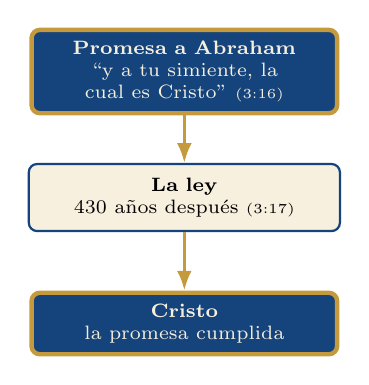
\begin{tikzpicture}[font=\scriptsize]
 \node[draw=dorado,line width=1.6pt,fill=azul,text=papiro,rounded corners=3pt,text width=3.6cm,align=center,inner sep=4pt] (a) at (0,1.6) {\textbf{Promesa a Abraham}\\ ``y a tu simiente, la cual es Cristo'' {\tiny(3:16)}};
 \node[caja,text width=3.6cm,align=center] (b) at (0,0) {\textbf{La ley}\\ 430 años después {\tiny(3:17)}};
 \node[draw=dorado,line width=1.6pt,fill=azul,text=papiro,rounded corners=3pt,text width=3.6cm,align=center,inner sep=4pt] (c) at (0,-1.6) {\textbf{Cristo}\\ la promesa cumplida};
 \draw[-{Latex[length=2.5mm]},dorado,line width=1.1pt](a)--(b); \draw[-{Latex[length=2.5mm]},dorado,line width=1.1pt](b)--(c);
\end{tikzpicture}\par\smallskip
\small Lo que Dios ratificó no se \destacar{invalida} (\grc{ἀθετεῖ}) ni se \destacar{abroga} (\grc{ἀκυροῖ}).
\end{column}
\end{columns}
\end{frame}

\begin{frame}{``No ha sido Sí y No''}
\begin{columns}[t,onlytextwidth]
\begin{column}{0.52\textwidth}
\begin{cita}Mas, como Dios es fiel, nuestra palabra a vosotros no es Sí y No. Porque el Hijo de Dios, Jesucristo\ldots{} no ha sido Sí y No; mas ha sido Sí en él; porque todas las promesas de Dios son en él Sí, y en él Amén.\fuente{(2 Co 1:18--20, RVR1960)}\end{cita}
\begin{cita}Si fuéremos infieles, él permanece fiel; él no puede negarse a sí mismo.\fuente{(2 Ti 2:13, RVR1960)}\end{cita}
\end{column}
\begin{column}{0.46\textwidth}\small
\begin{itemize}
\item Pablo, acusado de cambiar sus planes de viaje (2 Co 1:15--17), apela a la constancia de Dios.
\item En Cristo, Dios no dice ``sí'' hoy y ``no'' mañana: todas sus promesas son ``\destacar{Sí}''.
\item ``No puede negarse a sí mismo'': la fidelidad de Dios descansa en su \destacar{ser}.
\end{itemize}
\precision{la autoría paulina de 2 Timoteo se discute; la idea tiene respaldo en Ro 3:3--4: ``¿Su incredulidad habrá hecho nula la fidelidad de Dios? De ninguna manera''.}
\end{column}
\end{columns}
\end{frame}

\begin{frame}{¿Cambió Dios al hacerse hombre?}
\begin{columns}[t,onlytextwidth]
\begin{column}{0.50\textwidth}
\begin{cita}el cual, siendo en forma de Dios, no estimó el ser igual a Dios como cosa a que aferrarse, sino que se despojó a sí mismo, tomando forma de siervo, hecho semejante a los hombres.\fuente{(Flp 2:6--7, RVR1960)}\end{cita}
\scriptsize\grc{ὃς ἐν μορφῇ θεοῦ ὑπάρχων}: ``existiendo (continuamente) en forma de Dios''. \grc{ἐκένωσεν}: ``se vació''. \grc{λαβών}: ``tomando''.
\end{column}
\begin{column}{0.48\textwidth}\small
\begin{itemize}
\item Pablo no dice que el Hijo dejara de ser Dios: dice que \destacar{tomó} forma de siervo.
\item El Concilio de Calcedonia (451) confesó a Cristo en dos naturalezas ``sin confusión, \destacar{sin cambio} (\grc{ἀτρέπτως}), sin división, sin separación''.
\item \grc{ἀτρέπτως} es de la familia de \grc{τροπή} (Stg 1:17): ``sombra de variación''.
\end{itemize}
\precision{el sentido de \grc{ἐκένωσεν} se discute (``teorías kenóticas''); la lectura de Calcedonia es la clásica de la iglesia.}
\end{column}
\end{columns}
\end{frame}

\begin{frame}{La inmutabilidad de Dios, cumplida en Cristo}
\centering
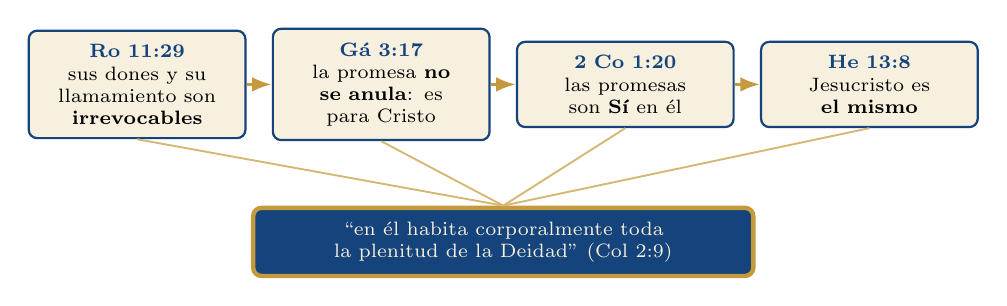
\begin{tikzpicture}[font=\scriptsize]
 \foreach \x/\y/\n/\t/\d in {0/0/a/{Ro 11:29}/{sus dones y su llamamiento son \textbf{irrevocables}},
   3.1/0/b/{Gá 3:17}/{la promesa \textbf{no se anula}: es para Cristo},
   6.2/0/c/{2 Co 1:20}/{las promesas son \textbf{Sí} en él},
   9.3/0/d/{He 13:8}/{Jesucristo es \textbf{el mismo}}}{
  \node[caja,text width=2.4cm,align=center] (\n) at (\x,\y) {\textbf{\textcolor{azul}{\t}}\\ \d};}
 \draw[-{Latex[length=2.5mm]},dorado,line width=1.1pt](a)--(b); \draw[-{Latex[length=2.5mm]},dorado,line width=1.1pt](b)--(c); \draw[-{Latex[length=2.5mm]},dorado,line width=1.1pt](c)--(d);
 \node[draw=dorado,line width=1.6pt,fill=azul,text=papiro,rounded corners=3pt,text width=6.0cm,align=center,inner sep=5pt] (e) at (4.65,-2.0) {``en él habita corporalmente toda la plenitud de la Deidad'' (Col 2:9)};
 \foreach \i in {a,b,c,d}\draw[dorado!70,line width=0.7pt](\i.south)--(e.north);
\end{tikzpicture}\par\medskip
\small\RaggedRight Pablo, judío formado en las Escrituras, lee el ``no cambio'' de Malaquías como \destacar{fidelidad de pacto cumplida en Cristo}. En él, el Dios que no cambia mostró su gloria ``en la faz de Jesucristo'' (2 Co 4:6), y en él el pueblo que cambia es ``transformado de gloria en gloria'' (2 Co 3:18).
\end{frame}

% ------------------------------------------------------------------
\section{Vivirlo}

\begin{frame}{Dónde pararnos con seguridad}
\begin{columns}[t,onlytextwidth]
\begin{column}{0.50\textwidth}
\begin{cita}Porque los montes se moverán, y los collados temblarán, pero no se apartará de ti mi misericordia, ni el pacto de mi paz se quebrantará, dijo \SENOR, el que tiene misericordia de ti.\fuente{(Is 54:10, RVR1960)}\end{cita}
\end{column}
\begin{column}{0.48\textwidth}\small
\textbf{Pink} (2020, cap. 7): ``No se puede confiar en la naturaleza humana; ¡pero sí se puede confiar en Dios!''. La multitud que gritó ``¡Hosanna!'' gritó después ``¡Crucifícale!''.\par\medskip
Pink cita a Charnock: ``¿Qué consuelo podríamos tener si orásemos a un dios que, como el camaleón, cambia de color continuamente?''.
\end{column}
\end{columns}\par\smallskip
\begin{tcolorbox}[colback=papiro,colframe=dorado,boxrule=1.2pt,arc=3pt]
\small La inmutabilidad ``tiene un lado oscuro y uno claro'': asegura ``la ejecución de sus amenazas, así como el cumplimiento de sus promesas'' (Dick, citado por Pink, 2020, cap. 7).
\end{tcolorbox}
\end{frame}

\begin{frame}{La oración: medio establecido por Dios}
\begin{columns}[t,onlytextwidth]
\begin{column}{0.50\textwidth}
\begin{cita}Vuélvete del ardor de tu ira, y arrepiéntete de este mal contra tu pueblo. Acuérdate de Abraham, de Isaac y de Israel tus siervos, a los cuales has jurado por ti mismo\ldots\fuente{(Éx 32:12--13, RVR1960)}\end{cita}
\end{column}
\begin{column}{0.48\textwidth}\small
\begin{itemize}
\item Moisés no pide a Dios que cambie de carácter: le pide que actúe \destacar{conforme} a su carácter y a su juramento.
\item Ora apoyado en lo que no cambia: ``a los cuales has jurado''.
\item Dios responde: ``Entonces \SENOR{} se arrepintió del mal'' (32:14).
\item Lo mismo Ezequías: ``Te ruego que te acuerdes'' (Is 38:3).
\end{itemize}
\end{column}
\end{columns}\par\smallskip
\small\RaggedRight Porque Dios no cambia, \destacar{orar tiene sentido}: se ora a alguien cuya palabra es firme y cuyo trato responde.
\end{frame}

\begin{frame}{Dios no cambia para que yo cambie}
\begin{columns}[t,onlytextwidth]
\begin{column}{0.50\textwidth}
\scriptsize\renewcommand{\arraystretch}{1.2}
\begin{tabular}{@{}>{\RaggedRight\arraybackslash}p{2.6cm}>{\RaggedRight\arraybackslash}p{3.1cm}@{}}
\toprule
\textbf{Lo que se pide} & \textbf{Texto} \\ \midrule
Volver a Dios & ``Volveos a mí, y yo me volveré a vosotros'' (Mal 3:7) \\
Ser transformado & ``somos transformados de gloria en gloria'' (2 Co 3:18) \\
No mudarse a otro evangelio & ``tan pronto os hayáis alejado'' (\grc{μετατίθεσθε}, Gá 1:6) \\
No fluctuar & ``que ya no seamos niños fluctuantes'' (Ef 4:14) \\
\bottomrule
\end{tabular}
\end{column}
\begin{column}{0.48\textwidth}
\begin{cita}Así que, hermanos míos amados, estad firmes y constantes, creciendo en la obra del Señor siempre, sabiendo que vuestro trabajo en el Señor no es en vano.\fuente{(1 Co 15:58, RVR1960)}\end{cita}
\scriptsize \grc{ἑδραῖοι\ldots{} ἀμετακίνητοι}: ``asentados\ldots{} inamovibles''. Pablo llama a la iglesia a reflejar, como criaturas, la firmeza de Dios.
\end{column}
\end{columns}
\end{frame}

\begin{frame}{Cuatro respuestas al Dios que no cambia}
\centering
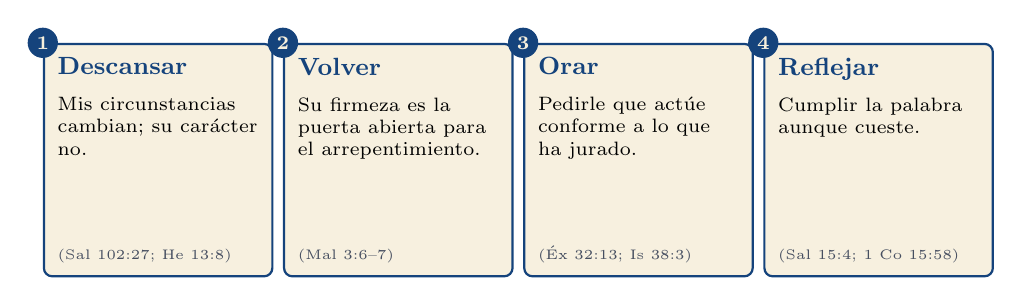
\begin{tikzpicture}
 \foreach \x/\n/\t/\d/\r in {0/1/{Descansar}/{Mis circunstancias cambian; su carácter no.}/{Sal 102:27; He 13:8},
   3.05/2/{Volver}/{Su firmeza es la puerta abierta para el arrepentimiento.}/{Mal 3:6--7},
   6.1/3/{Orar}/{Pedirle que actúe conforme a lo que ha jurado.}/{Éx 32:13; Is 38:3},
   9.15/4/{Reflejar}/{Cumplir la palabra aunque cueste.}/{Sal 15:4; 1 Co 15:58}}{
  \node[caja,anchor=north] (b\n) at (\x,0) {\parbox[t][2.6cm][t]{2.55cm}{\RaggedRight
    {\small\textbf{\textcolor{azul}{\t}}}\\[5pt]\scriptsize \d\par\vfill{\tiny\color{gris}(\r)}}};
  \node[circle,fill=azul,text=papiro,font=\scriptsize\bfseries,inner sep=1.6pt] at (b\n.north west) {\n};}
\end{tikzpicture}\par\medskip
\begin{cita}El que aun jurando en daño suyo, no por eso cambia.\fuente{(Sal 15:4c, RVR1960)}\end{cita}
\centering\heb{נִשְׁבַּע לְהָרַע וְלֹא יָמִר}
\end{frame}

% ------------------------------------------------------------------
\section{Síntesis}

\begin{frame}{Síntesis}
\begin{tcolorbox}[colback=papiro,colframe=azul,boxrule=1pt,arc=3pt]
\small ``Porque yo \SENOR{} no cambio; por esto, hijos de Jacob, no habéis sido consumidos'' (Mal 3:6). Dios es eternamente \destacar{el mismo} en su ser, su carácter y sus atributos; por eso su pueblo no se acaba. Su ``arrepentirse'' no es error ni capricho, sino la respuesta \destacar{coherente} de un carácter que no cambia: desiste del mal ante el que se vuelve (Jer 18:8; Jon 3:10) y nunca revoca lo que juró (Nm 23:19; Sal 110:4). En Cristo, sus dones son irrevocables (Ro 11:29), sus promesas son Sí (2 Co 1:20), y Jesucristo es el mismo ayer, y hoy, y por los siglos (He 13:8).
\end{tcolorbox}
\scriptsize\renewcommand{\arraystretch}{1.13}
\begin{tabular}{@{}>{\RaggedRight\arraybackslash}p{2.0cm}>{\RaggedRight\arraybackslash}p{9.8cm}@{}}
\toprule
\textbf{Mirada} & \textbf{Aporte} \\ \midrule
Hebrea & \emph{lo shaníti} (Mal 3:6); \emph{atá hu} (Sal 102:27); la Roca de los siglos; \emph{najam} como cambio de trato; Jer 18; Balaam. \\
Judía & \emph{Atá hu} y \emph{Adón olam}; \emph{Ehyé} = ``estaré con ellos''; los targumes; Rashi y \emph{Bereshit Rabá} 27:4; \emph{Rosh Hashaná} 16b; Filón y Maimónides. \\
Pink & inmutable en esencia, atributos y consejo; la Roca; ``criatura y mutabilidad son términos correlativos''. \\
Paulina & dones irrevocables; la promesa que la ley no anula; el Sí de Dios en Cristo; el Dios incorruptible; firmes y constantes. \\
\bottomrule
\end{tabular}
\end{frame}

\begin{frame}{Para la reflexión}
\begin{cita}Mas alábese en esto el que se hubiere de alabar: en entenderme y conocerme, que yo soy \SENOR, que hago misericordia, juicio y justicia en la tierra; porque estas cosas quiero, dice \SENOR.\fuente{(Jer 9:24 [9:23], RVR1960)}\end{cita}
\begin{center}\heb{כִּי אֲנִי יְהוָה עֹשֶׂה חֶסֶד מִשְׁפָּט וּצְדָקָה בָּאָרֶץ}\end{center}
\small
\begin{itemize}
\item ¿Pienso en Dios como un ser inmóvil y distante, o como el que es siempre el mismo \emph{conmigo}?
\item ¿Confío más en las circunstancias, en las personas o en la Roca?
\item ¿Qué ``juicio anunciado'' en mi vida me llama a volver (Mal 3:7)?
\item ¿Oro apoyado en lo que Dios ha jurado?
\end{itemize}
\end{frame}

% ------------------------------------------------------------------
\section{Glosario}

\begin{frame}{Glosario}
\scriptsize
\begin{columns}[t,onlytextwidth]
\begin{column}{0.49\textwidth}
\begin{description}\setlength{\itemsep}{1pt}
\item[\emph{Ametamélētos}] (\grc{ἀμεταμέλητος}) sin vuelta atrás; ``irrevocable'' (Ro 11:29).
\item[\emph{Ametáthetos}] (\grc{ἀμετάθετος}) que no se traslada; ``inmutable'' (He 6:17--18).
\item[\emph{Áphthartos}] (\grc{ἄφθαρτος}) incorruptible (Ro 1:23; 1 Ti 1:17).
\item[\emph{Atá hu}] (\heb{אַתָּה הוּא}) ``tú eres él'': ``tú eres el mismo'' (Sal 102:27).
\item[\emph{Atréptōs}] (\grc{ἀτρέπτως}) ``sin cambio'' (Calcedonia, 451).
\item[\emph{Ehyé}] (\heb{אֶהְיֶה}) ``soy / seré / estaré'' (Éx 3:12, 14).
\item[\emph{Jalaf}] (\heb{חָלַף}) pasar; mudar (ropa) (Sal 102:26).
\item[\emph{Memrá}] (\heb{מֵימְרָא}) ``Palabra'' del \SENOR{} en los targumes.
\end{description}
\end{column}
\begin{column}{0.49\textwidth}
\begin{description}\setlength{\itemsep}{1pt}
\item[\emph{Najam}] (\heb{נחם}) lamentar, compadecerse, desistir; consolar.
\item[\emph{Nétsaj}] (\heb{נֵצַח}) perpetuidad, gloria; ``la Gloria de Israel'' (1 S 15:29).
\item[\emph{Nimlaj}] (\heb{נִמְלָךְ}) ``deliberar'' (Rashi sobre \emph{najam}).
\item[\emph{Ho autós}] (\grc{ὁ αὐτός}) ``el mismo'' (He 1:12; 13:8).
\item[\emph{Shaná}] (\heb{שָׁנָה}) cambiar; repetir (Mal 3:6).
\item[\emph{Shinui maasé}] (\heb{שִׁינּוּי מַעֲשֶׂה}) cambio de conducta (\emph{Rosh Hashaná} 16b).
\item[\emph{Tropé}] (\grc{τροπή}) giro, variación (Stg 1:17).
\item[\emph{Tsur}] (\heb{צוּר}) roca (Dt 32:4); \emph{tsur olamim}, ``Roca de los siglos'' (Is 26:4).
\end{description}
\end{column}
\end{columns}
\end{frame}

% ------------------------------------------------------------------
\section{Referencias}

\begin{frame}{Referencias}
\fontsize{5.4}{6.4}\selectfont
\begin{columns}[t,onlytextwidth]
\begin{column}{0.49\textwidth}
\refapa{Bauer, W., Danker, F.~W., Arndt, W.~F., \& Gingrich, F.~W. (2000). \emph{A Greek-English lexicon of the New Testament and other early Christian literature} (3.ª ed.). University of Chicago Press.}
\refapa{\emph{Bereshit Rabá} [27:4]. (2022). (The Sefaria Midrash Rabbah). Sefaria. https://www.sefaria.org}
\refapa{Brown, F., Driver, S.~R., \& Briggs, C.~A. (1906). \emph{A Hebrew and English lexicon of the Old Testament}. Clarendon Press.}
\refapa{Denzinger, H., \& Hünermann, P. (Eds.). (2012). \emph{Enchiridion symbolorum, definitionum et declarationum de rebus fidei et morum} (43.ª ed.). Ignatius Press. [Calcedonia, DH 302]}
\refapa{Elliger, K., \& Rudolph, W. (Eds.). (1997). \emph{Biblia Hebraica Stuttgartensia} (5.ª ed.). Deutsche Bibelgesellschaft.}
\refapa{Fee, G.~D. (1987). \emph{The first epistle to the Corinthians}. Eerdmans.}
\refapa{Filón de Alejandría. (1993). Sobre la inmutabilidad de Dios [\emph{Quod Deus sit immutabilis}]. En \emph{The works of Philo} (C.~D. Yonge, Trad.). Hendrickson. (Obra original del s.~I)}
\refapa{García Martínez, F. (1992). \emph{Textos de Qumrán}. Trotta.}
\refapa{Koehler, L., \& Baumgartner, W. (2001). \emph{The Hebrew and Aramaic lexicon of the Old Testament} (Ed. de estudio). Brill.}
\refapa{Maimónides. (s.f.). \emph{Mishné Torá: Yesodé haTorá} [1:11--12]. Sefaria. https://www.sefaria.org}
\refapa{\emph{Misná: Taanit} [2:1]. (s.f.). Sefaria. https://www.sefaria.org}
\refapa{Nestle, E., \& Aland, K. (Eds.). (2012). \emph{Novum Testamentum Graece} (28.ª ed.). Deutsche Bibelgesellschaft.}
\end{column}
\begin{column}{0.49\textwidth}
\refapa{Pink, A.~W. (2020). \emph{Los atributos de Dios} (E. Rodríguez Cruz, Trad.). Chapel Library. (Obra original publicada en 1930)}
\refapa{Platón. (1930). \emph{The Republic} (P. Shorey, Trad.; Vol. 1). Harvard University Press. [II, 381c]}
\refapa{Rahlfs, A., \& Hanhart, R. (Eds.). (2006). \emph{Septuaginta} (Ed. rev.). Deutsche Bibelgesellschaft.}
\refapa{Rashi. (s.f.). \emph{Comentario a Génesis, Éxodo, Números, 1 Samuel y Malaquías} [Gn 6:6; Éx 3:14; Nm 23:19; 1 S 15:29; Mal 3:6]. Sefaria. https://www.sefaria.org}
\refapa{\emph{Santa Biblia: Reina-Valera 1960}. (1960). Sociedades Bíblicas en América Latina.}
\refapa{\emph{Shemot Rabá} [3:6]. (s.f.). Sefaria. https://www.sefaria.org}
\refapa{\emph{Sidur Ashkenaz} [Shajarit; \emph{Adón olam}]. (s.f.). Sefaria. https://www.sefaria.org}
\refapa{Steinsaltz, A. (Ed.). (2017). \emph{Koren Talmud Bavli: Edición William Davidson} [Berajot 9b; Rosh Hashaná 16b; Sotá 9a]. Sefaria. https://www.sefaria.org}
\refapa{Strong, J. (1890). \emph{The exhaustive concordance of the Bible}. Hunt \& Eaton.}
\refapa{\emph{Targum Jonatán a los Profetas} [1 S 15:29]; \emph{Targum Ónkelos} [Gn 6:6; Nm 23:19]. (s.f.). Sefaria. https://www.sefaria.org}
\refapa{Vermes, G. (2004). \emph{The complete Dead Sea Scrolls in English} (Ed. rev.). Penguin.}
\refapa{Vine, W.~E. (1999). \emph{Diccionario expositivo de palabras del Antiguo y del Nuevo Testamento exhaustivo}. Caribe.}
\end{column}
\end{columns}
\par\smallskip{\color{gris}Las citas bíblicas son de la Reina-Valera 1960; ``Jehová'' se reemplaza por \SENOR. Hebreo: BHS; griego: NA28 y LXX de Rahlfs-Hanhart. Fuentes judías: Sefaria; lo rabínico se marca como \emph{precisión}.}
\end{frame}

\end{document}
